\message{ !name(latexworkhop_report.tex)}\documentclass[a4paper,12pt]{report}

% Page Layout
\usepackage{geometry}
\geometry{
  a4paper,
  left=20mm,
  right=20mm,
  bottom=15mm,
  top=15mm
}
\usepackage{Archivo}
\usepackage[T1]{fontenc}
\sffamily

\usepackage{subcaption}
\usepackage{graphicx, wrapfig, xcolor, multicol}
\usepackage{tikz, pgfplots}
\usepgflibrary{shadings}
\usetikzlibrary{positioning, shapes.geometric, fit}
\pgfplotsset{compat=1.18}
\usepackage{amsmath, amssymb, amsthm, mathtools}
\usepackage[most]{tcolorbox}
\graphicspath{{images/}}

\linespread{1.3}
\usepackage{url}
\urlstyle{same}
\usepackage{hyperref}
\hypersetup{
    colorlinks=true,
    linkcolor=blue,
    filecolor=magenta,
    urlcolor=cyan,
  }


% ------------------------------------------------------------------------------------------------------------------
\begin{document}

\message{ !name(latexworkhop_report.tex) !offset(103) }
cheifguest.jpg}
    \caption{Chief Guest Dr. Ishwar Koirala}
    \label{fig:first}
\end{subfigure}
\hfill
\begin{subfigure}{0.42\textwidth}
    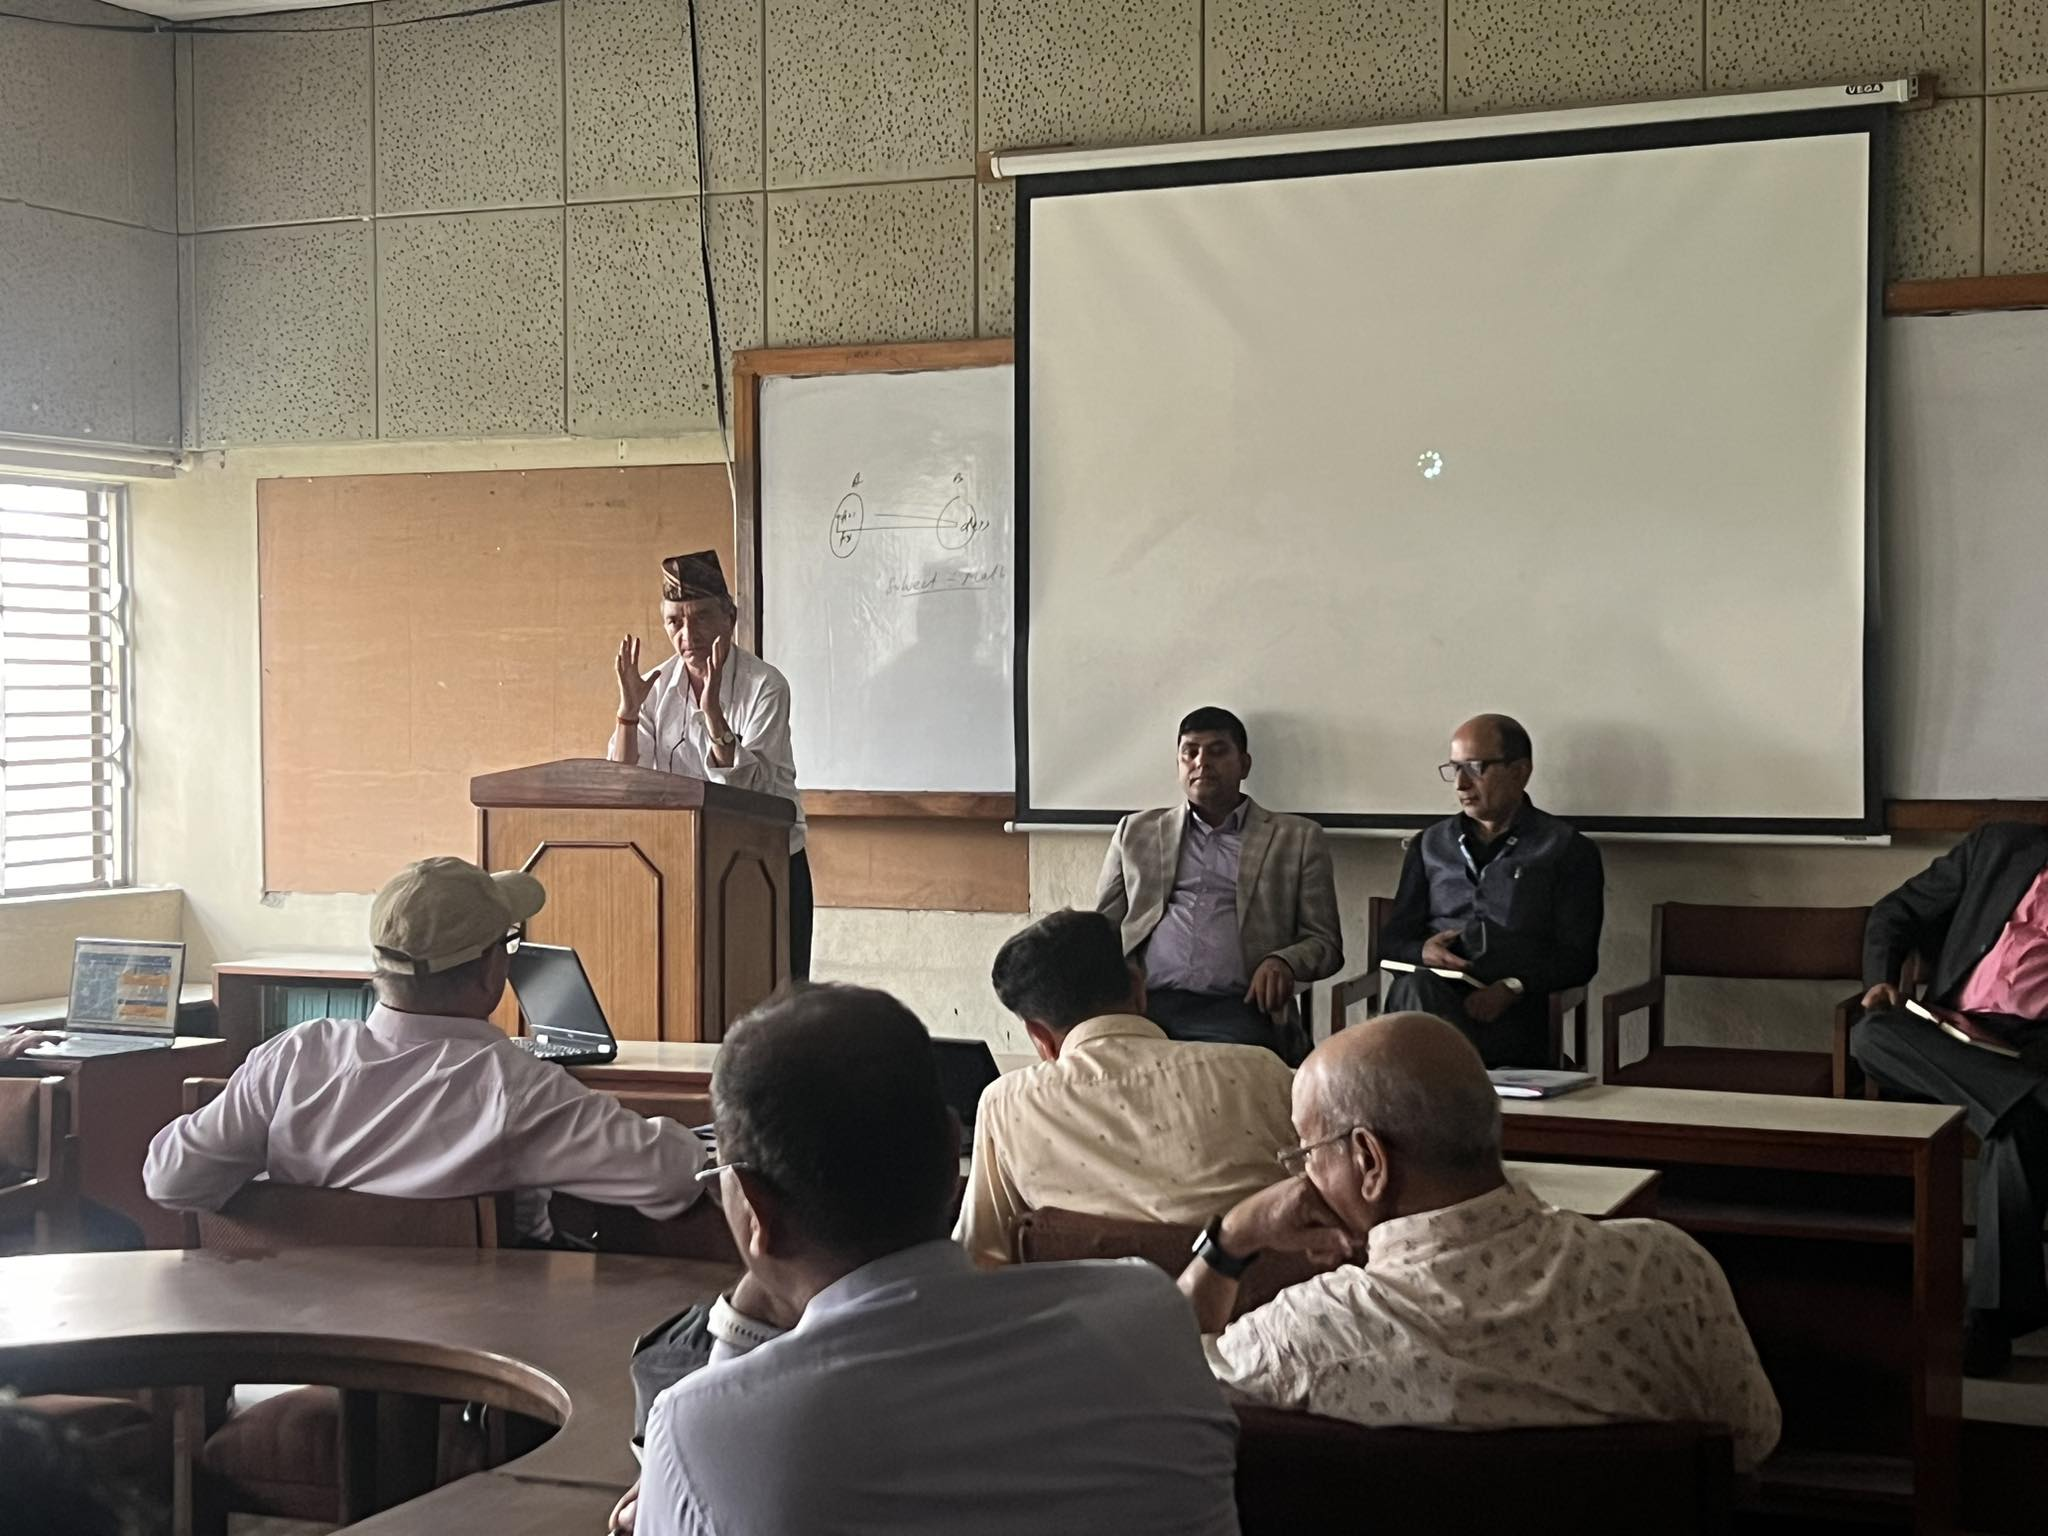
\includegraphics[height=7cm, width=\textwidth]{chet.jpg}
    \caption{Chairman Dr. Bhatta}
    \label{fig:second}
\end{subfigure}
\end{figure}

\vspace{5mm}
\noindent
The Chairman of the workshop HoD Prof. Dr. {Chet Raj Bhatta} praised and thanked the coordinator of the workshop Dr. Kafle for his dedication and hard work in making this workshop happen. He also thanked the whole organizing team for their support and hard work. He welcomed all the guests and participants and gave his best wishes for the success of the workshop. He asked every participants to make the best out of this workshop and learn as much as possible and share their knowledge to others as well after the completion of the workshop.
\clearpage


\vspace*{5mm}
\begin{figure}[h!]
\centering
\begin{subfigure}{0.45\textwidth}
    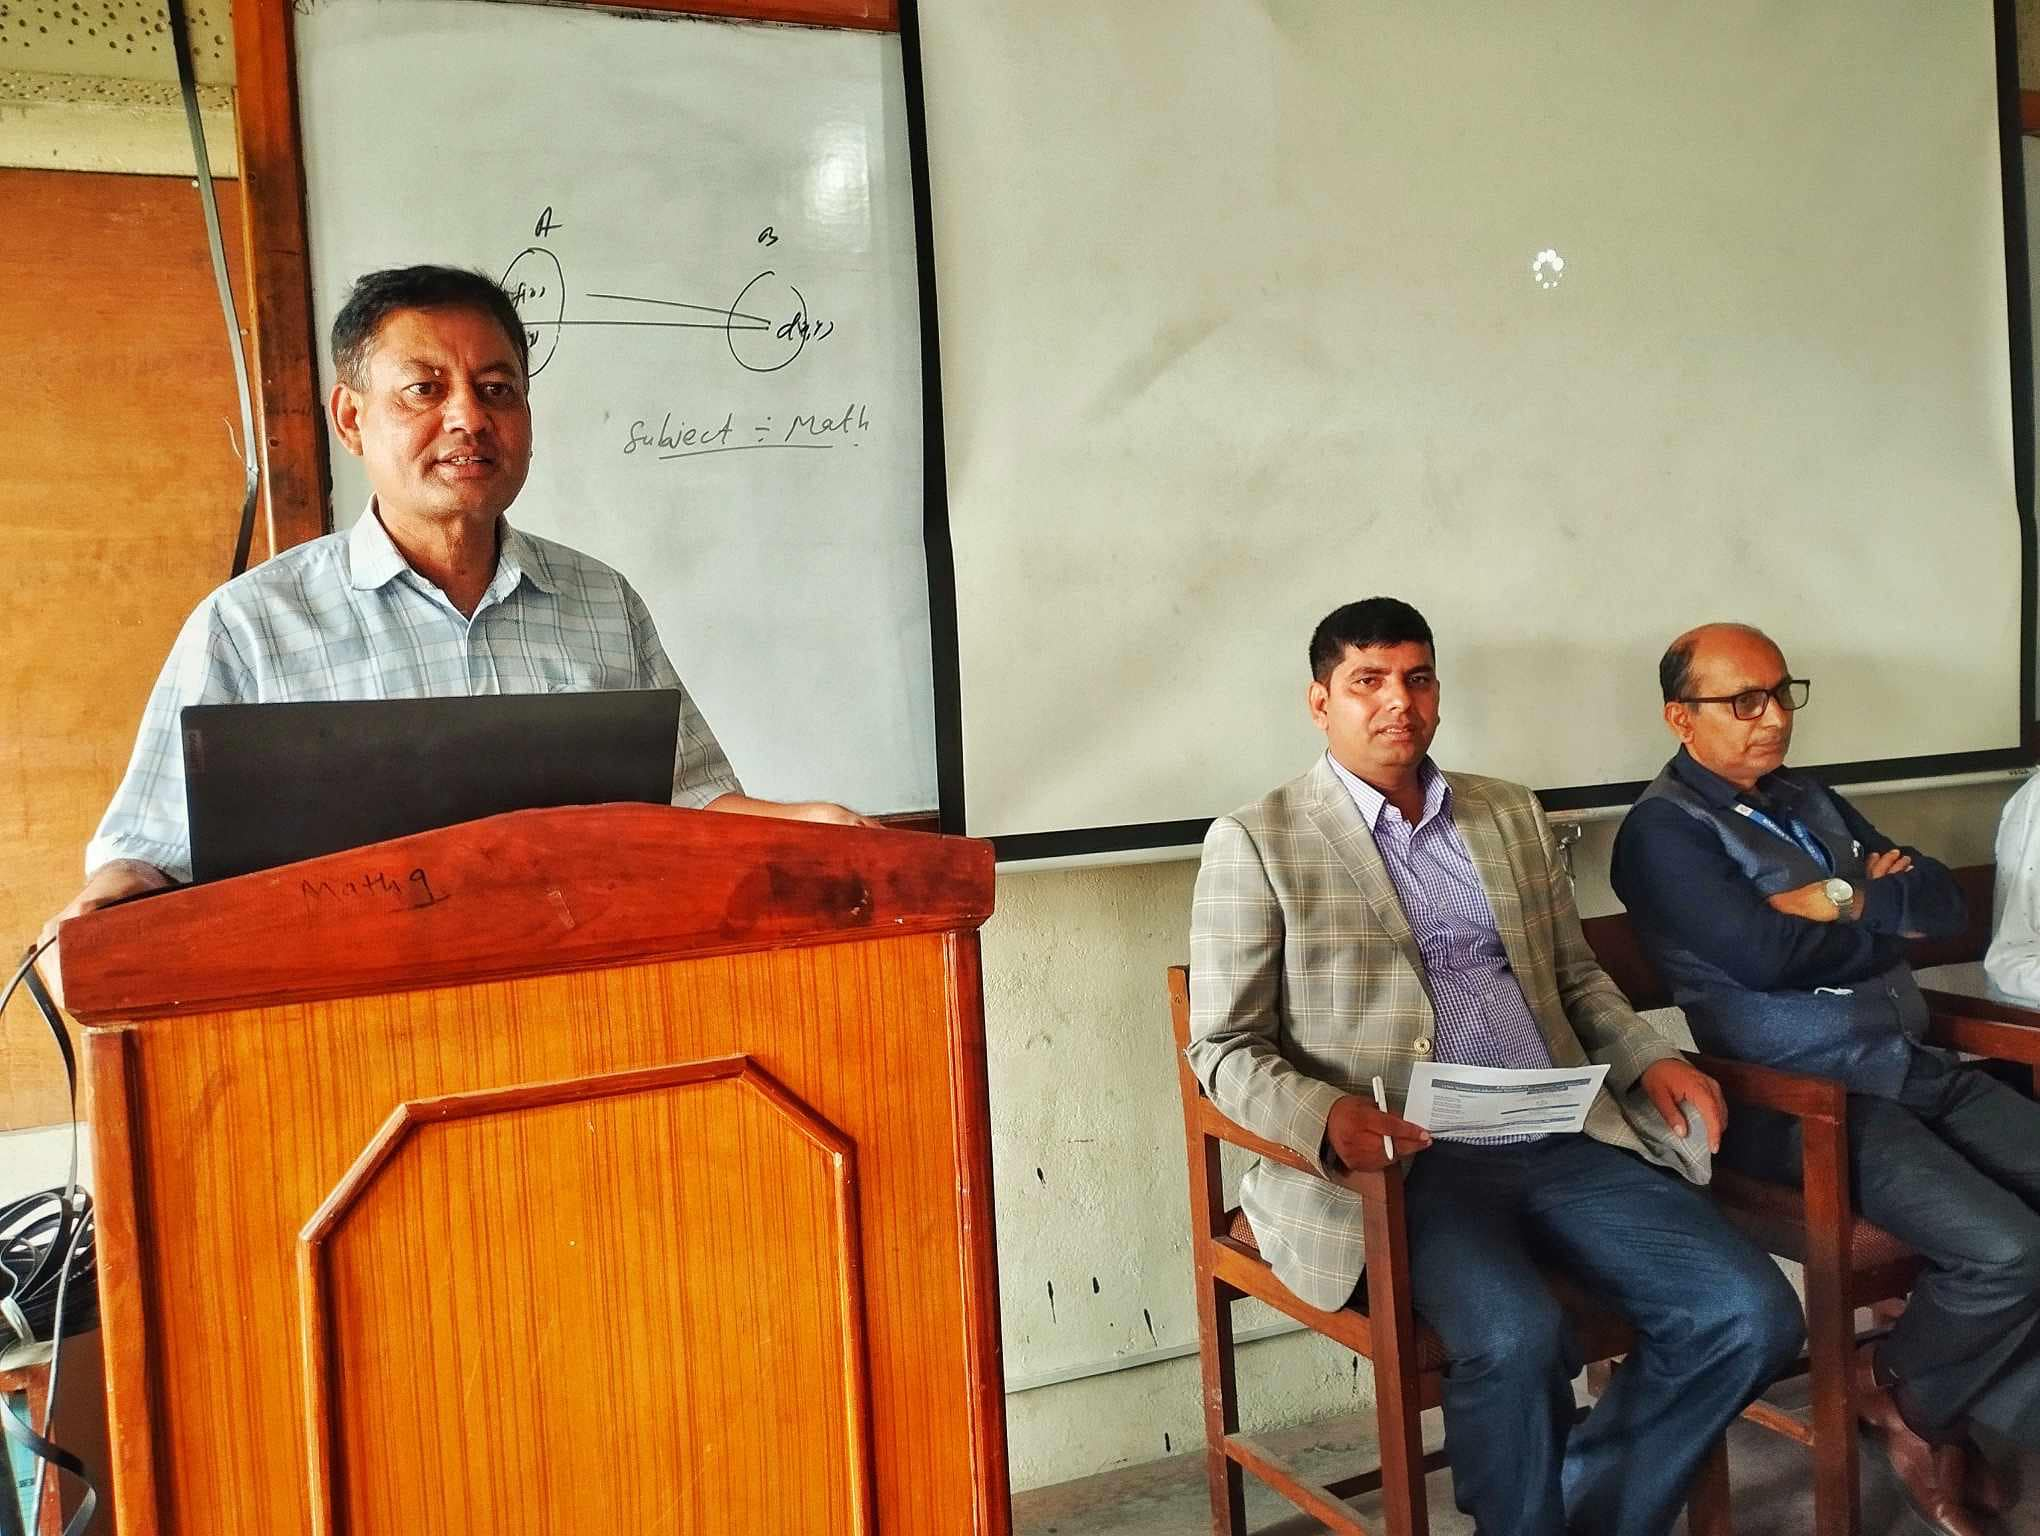
\includegraphics[height=7cm, width=\textwidth]{shreeramsir.jpg}
    \caption{Dr. Khadka}
    \label{fig:first}
\end{subfigure}
\hfill
\begin{subfigure}{0.45\textwidth}
    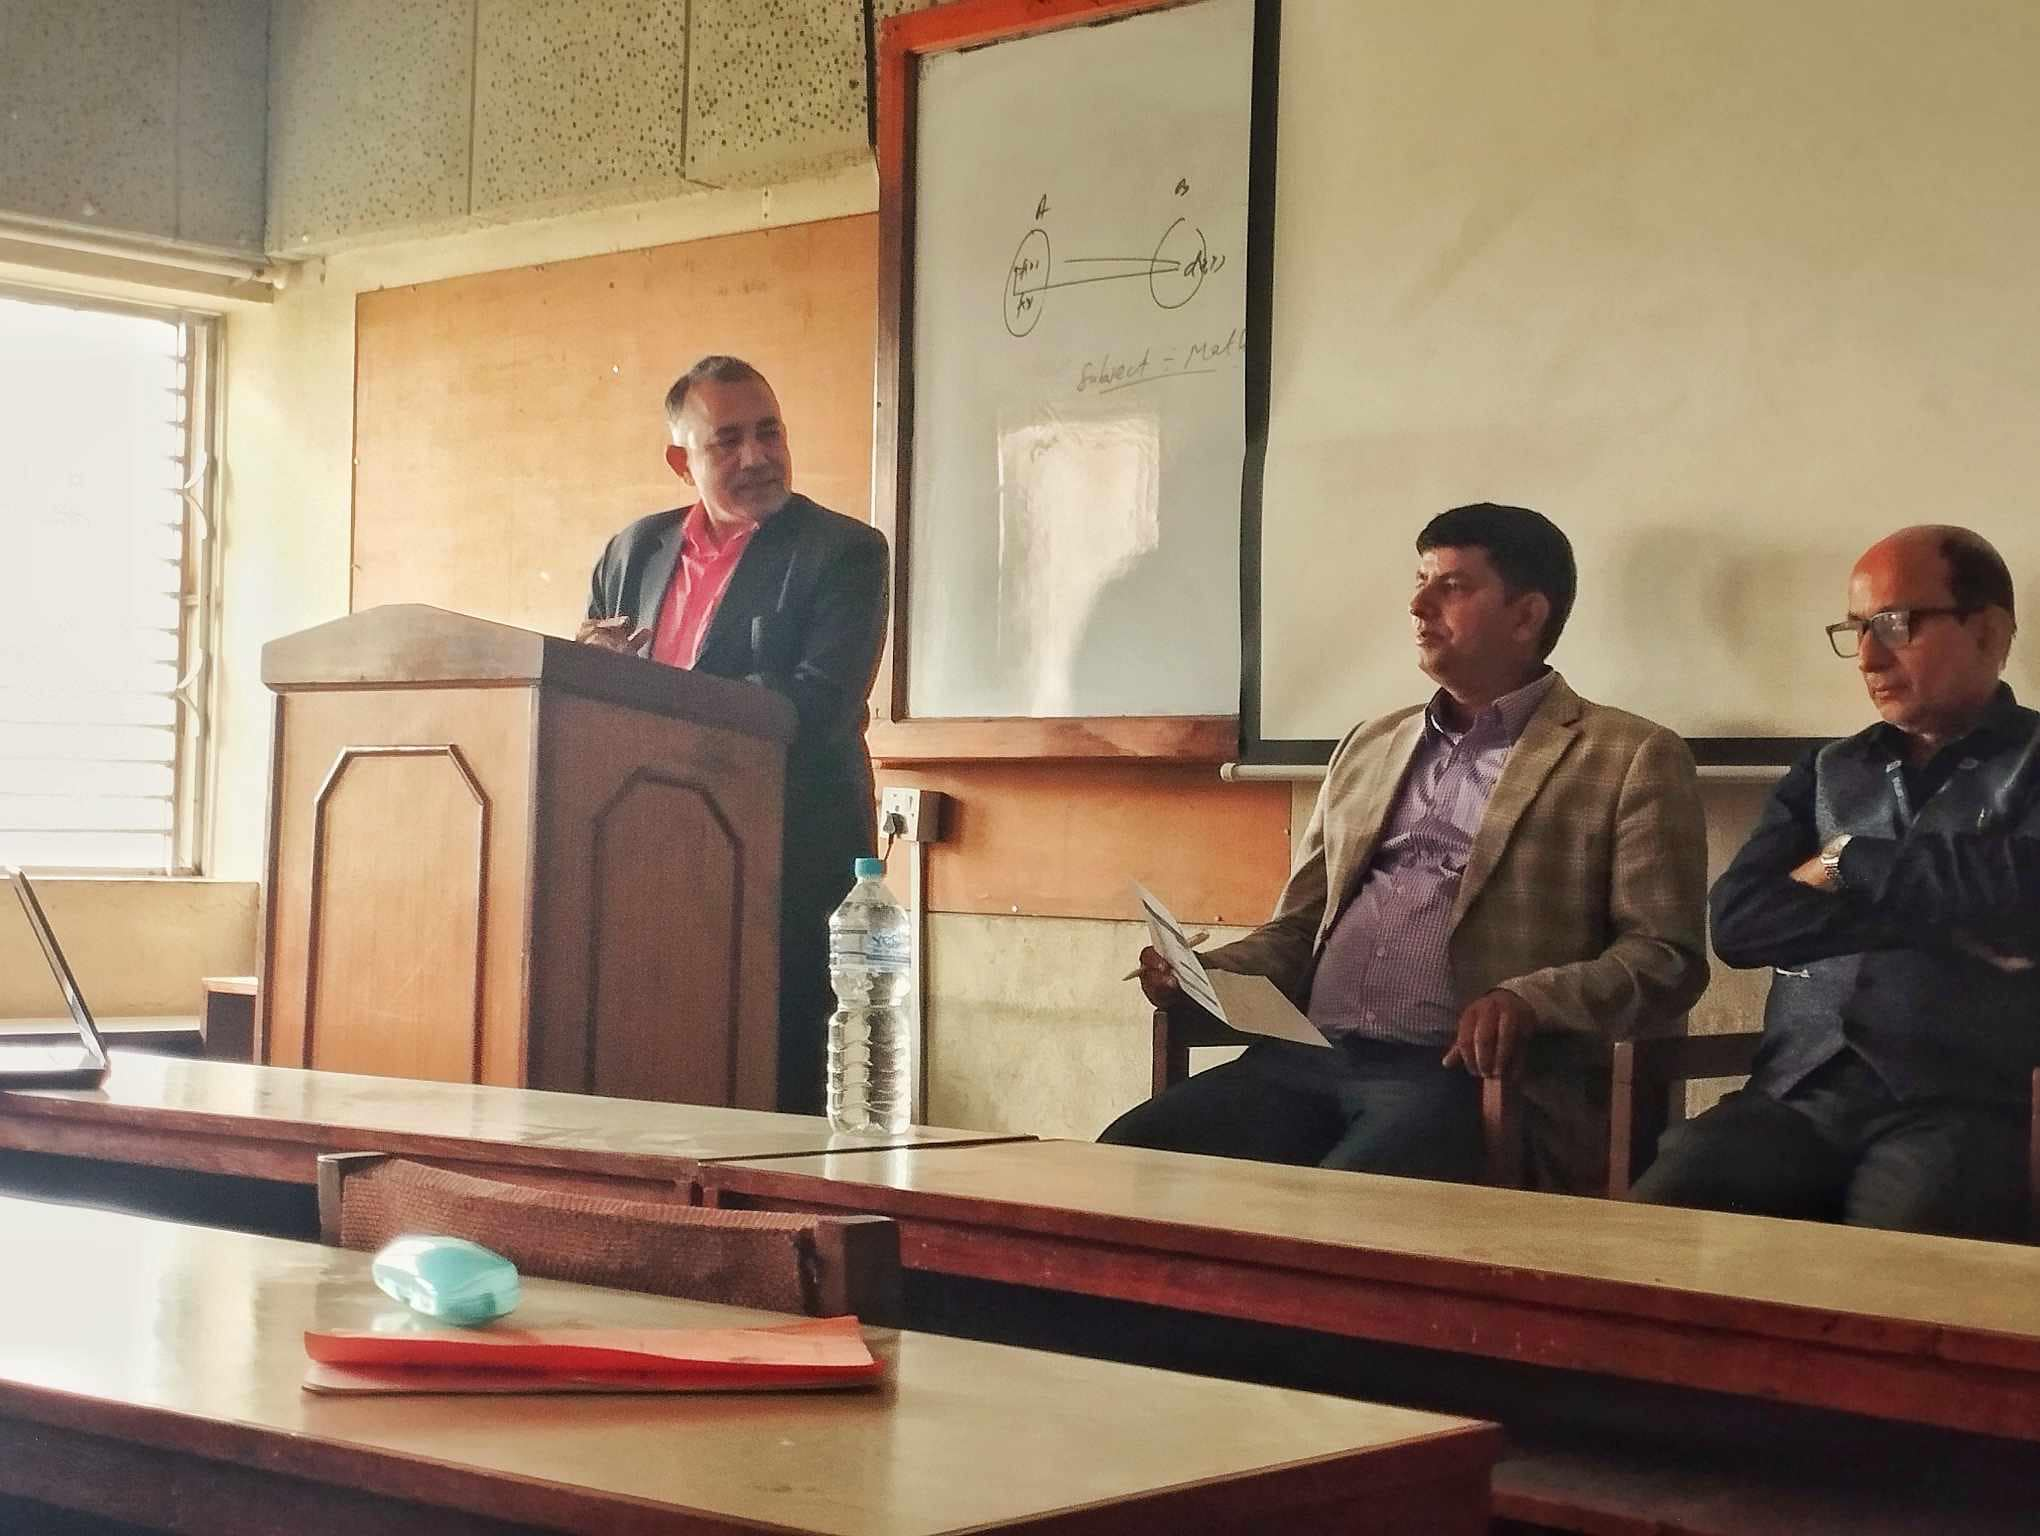
\includegraphics[height=7cm, width=\textwidth]{gyansir.jpg}
    \caption{Dr. Thapa}
    \label{fig:second}
\end{subfigure}
\end{figure}

\noindent
The vice-president of Nepal Mathematical Society Assoc. Prof. Dr. \textbf{Shree Ram Khadka} spoke about the importance of such workshops and gave a big encouragement to the participants and the organizing team.The he made the participants known about the recently added new grants by the Society to the Mphil and Phd Scholars. The president of the CDM alumni association Prof. Dr. {Gyan Bahadur Thapa} said such interactions help increase in the member of the association and gave his best wishes to the success of the workshop.\\[3mm]

The newly appointed vice-principal of the Pulchowk Campus, IoST, TU Dr.\textbf{ Puskar Raj Pokharel} said latex can be difficult learn in the beginning and talked about the challenges of learning latex in old times when there was good internet and technology. He also talked about the advantages of using latex which is a powerful markup languages over word-processors as MS-word. Latex has significant advantages in typesetting math symbols over the word-processors.

\begin{figure}[h!]
  \centering
  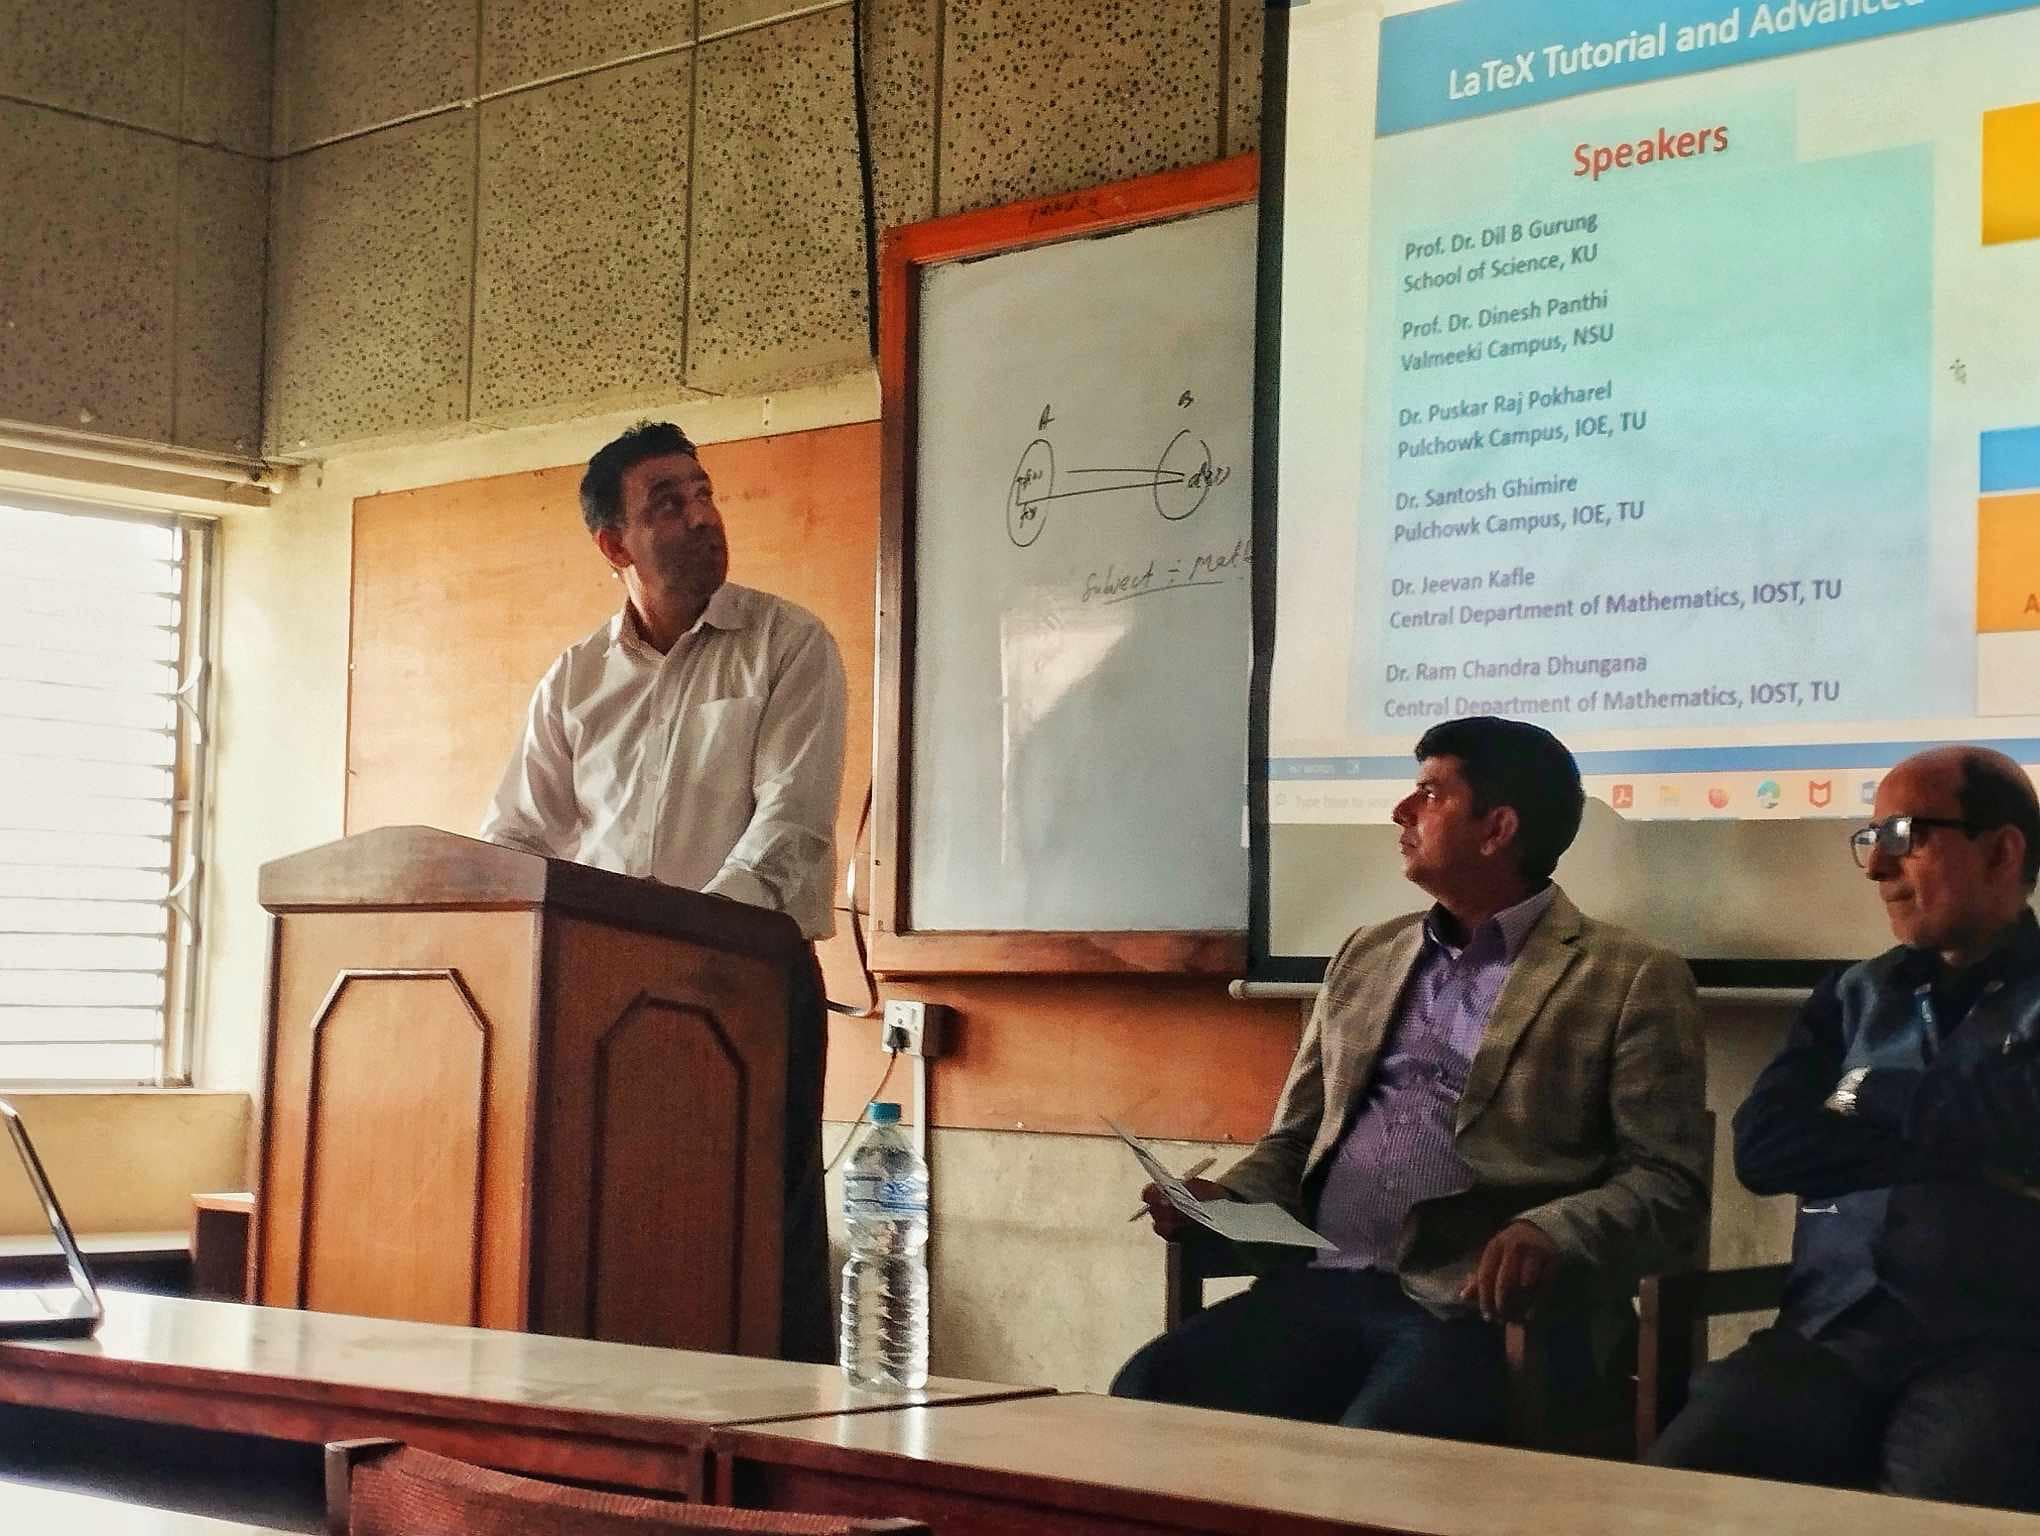
\includegraphics[height=6cm, width=9cm]{puskarsir2.jpg}
  \caption{Dr. Puskar Raj Pokharel}
\end{figure}
\clearpage

\begin{center}
  {\bfseries \Large Day 1, 20-Baishakh, Thursday}
\end{center}
\vspace{3mm}

{\bfseries \large Sessioin 1}\\[3mm]
The first expert of this session was Dr. \textbf{Ram Chandra Dhungana} and Dr. \textbf{Kafle}. Dr. Dhungana trained the participants on the \textit{Basics of Latex, Creation of a Latex document and Mathematics in Latex}.
\vspace{3mm}

\begin{figure}[h!]
  \centering
  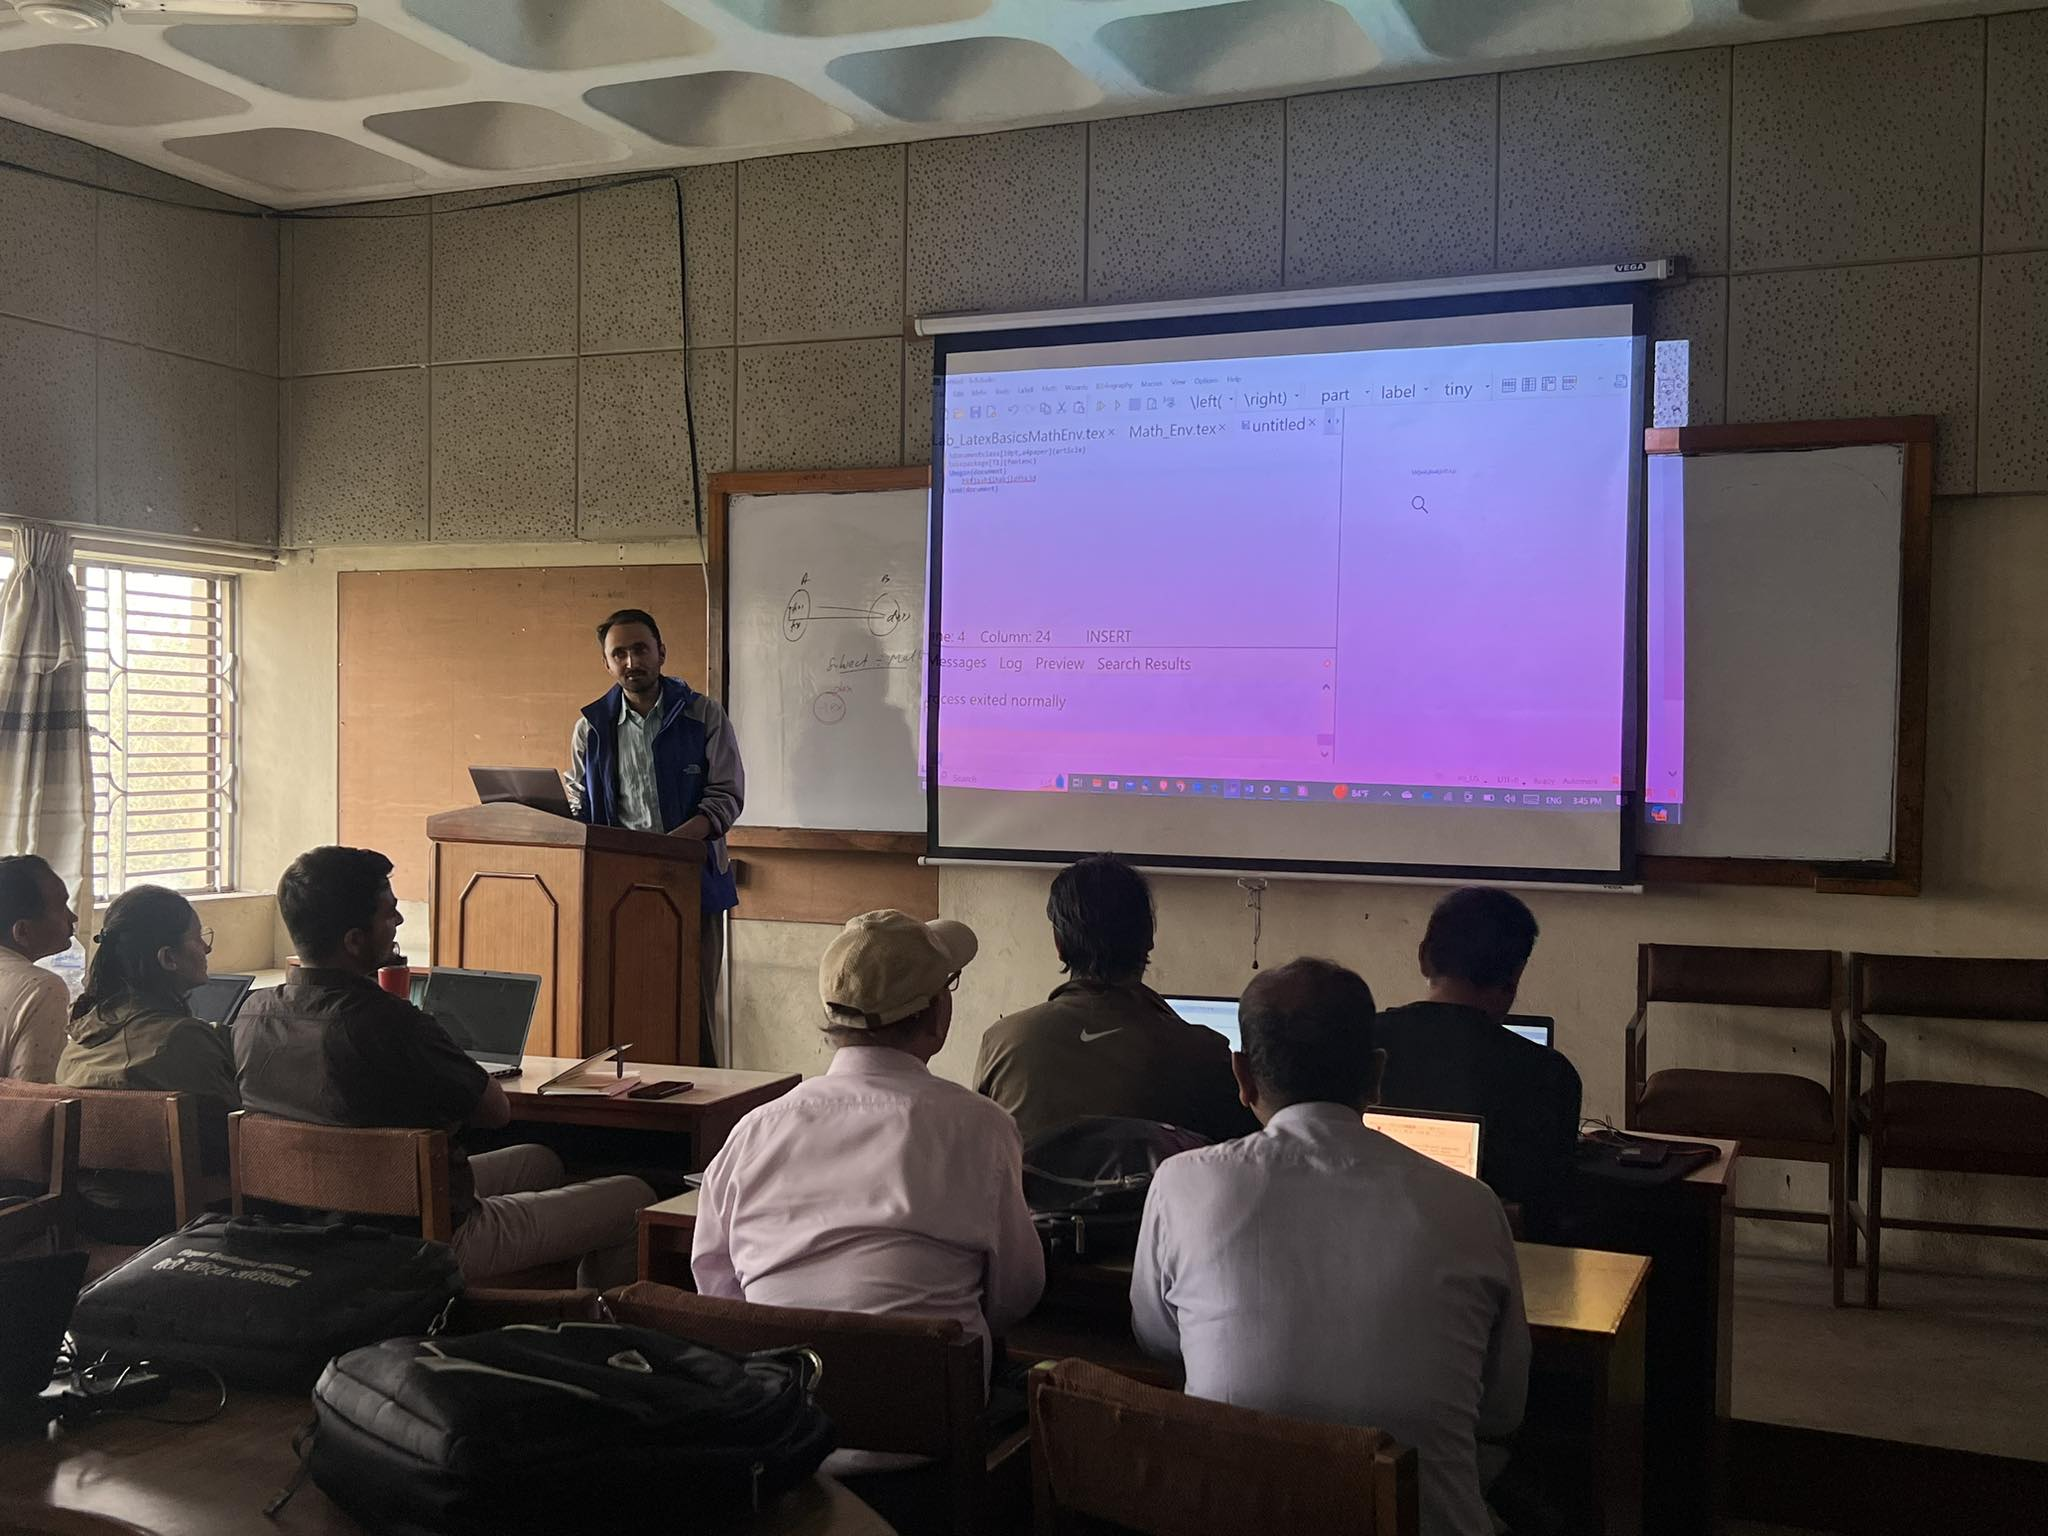
\includegraphics[height=7cm, width=9cm]{rcd.jpg}
  \caption{Dr. Ram Chandra Dhungana}
\end{figure}
\vspace{2mm}
The workshop broke for snacks at 5:30pm.

\vspace{5mm}

{\bfseries \large Session 2}\\[3mm]
The expert of this session was the vice-principal of Pulchowok Campus, Dr. \textbf{Puskar Raj Pokharel}. He trained the participants on the two important aspects of latex document \textit{Including Graphs and Placing Figures and Preparing Bibliography}.
\vspace{3mm}

\begin{figure}[h!]
  \centering
  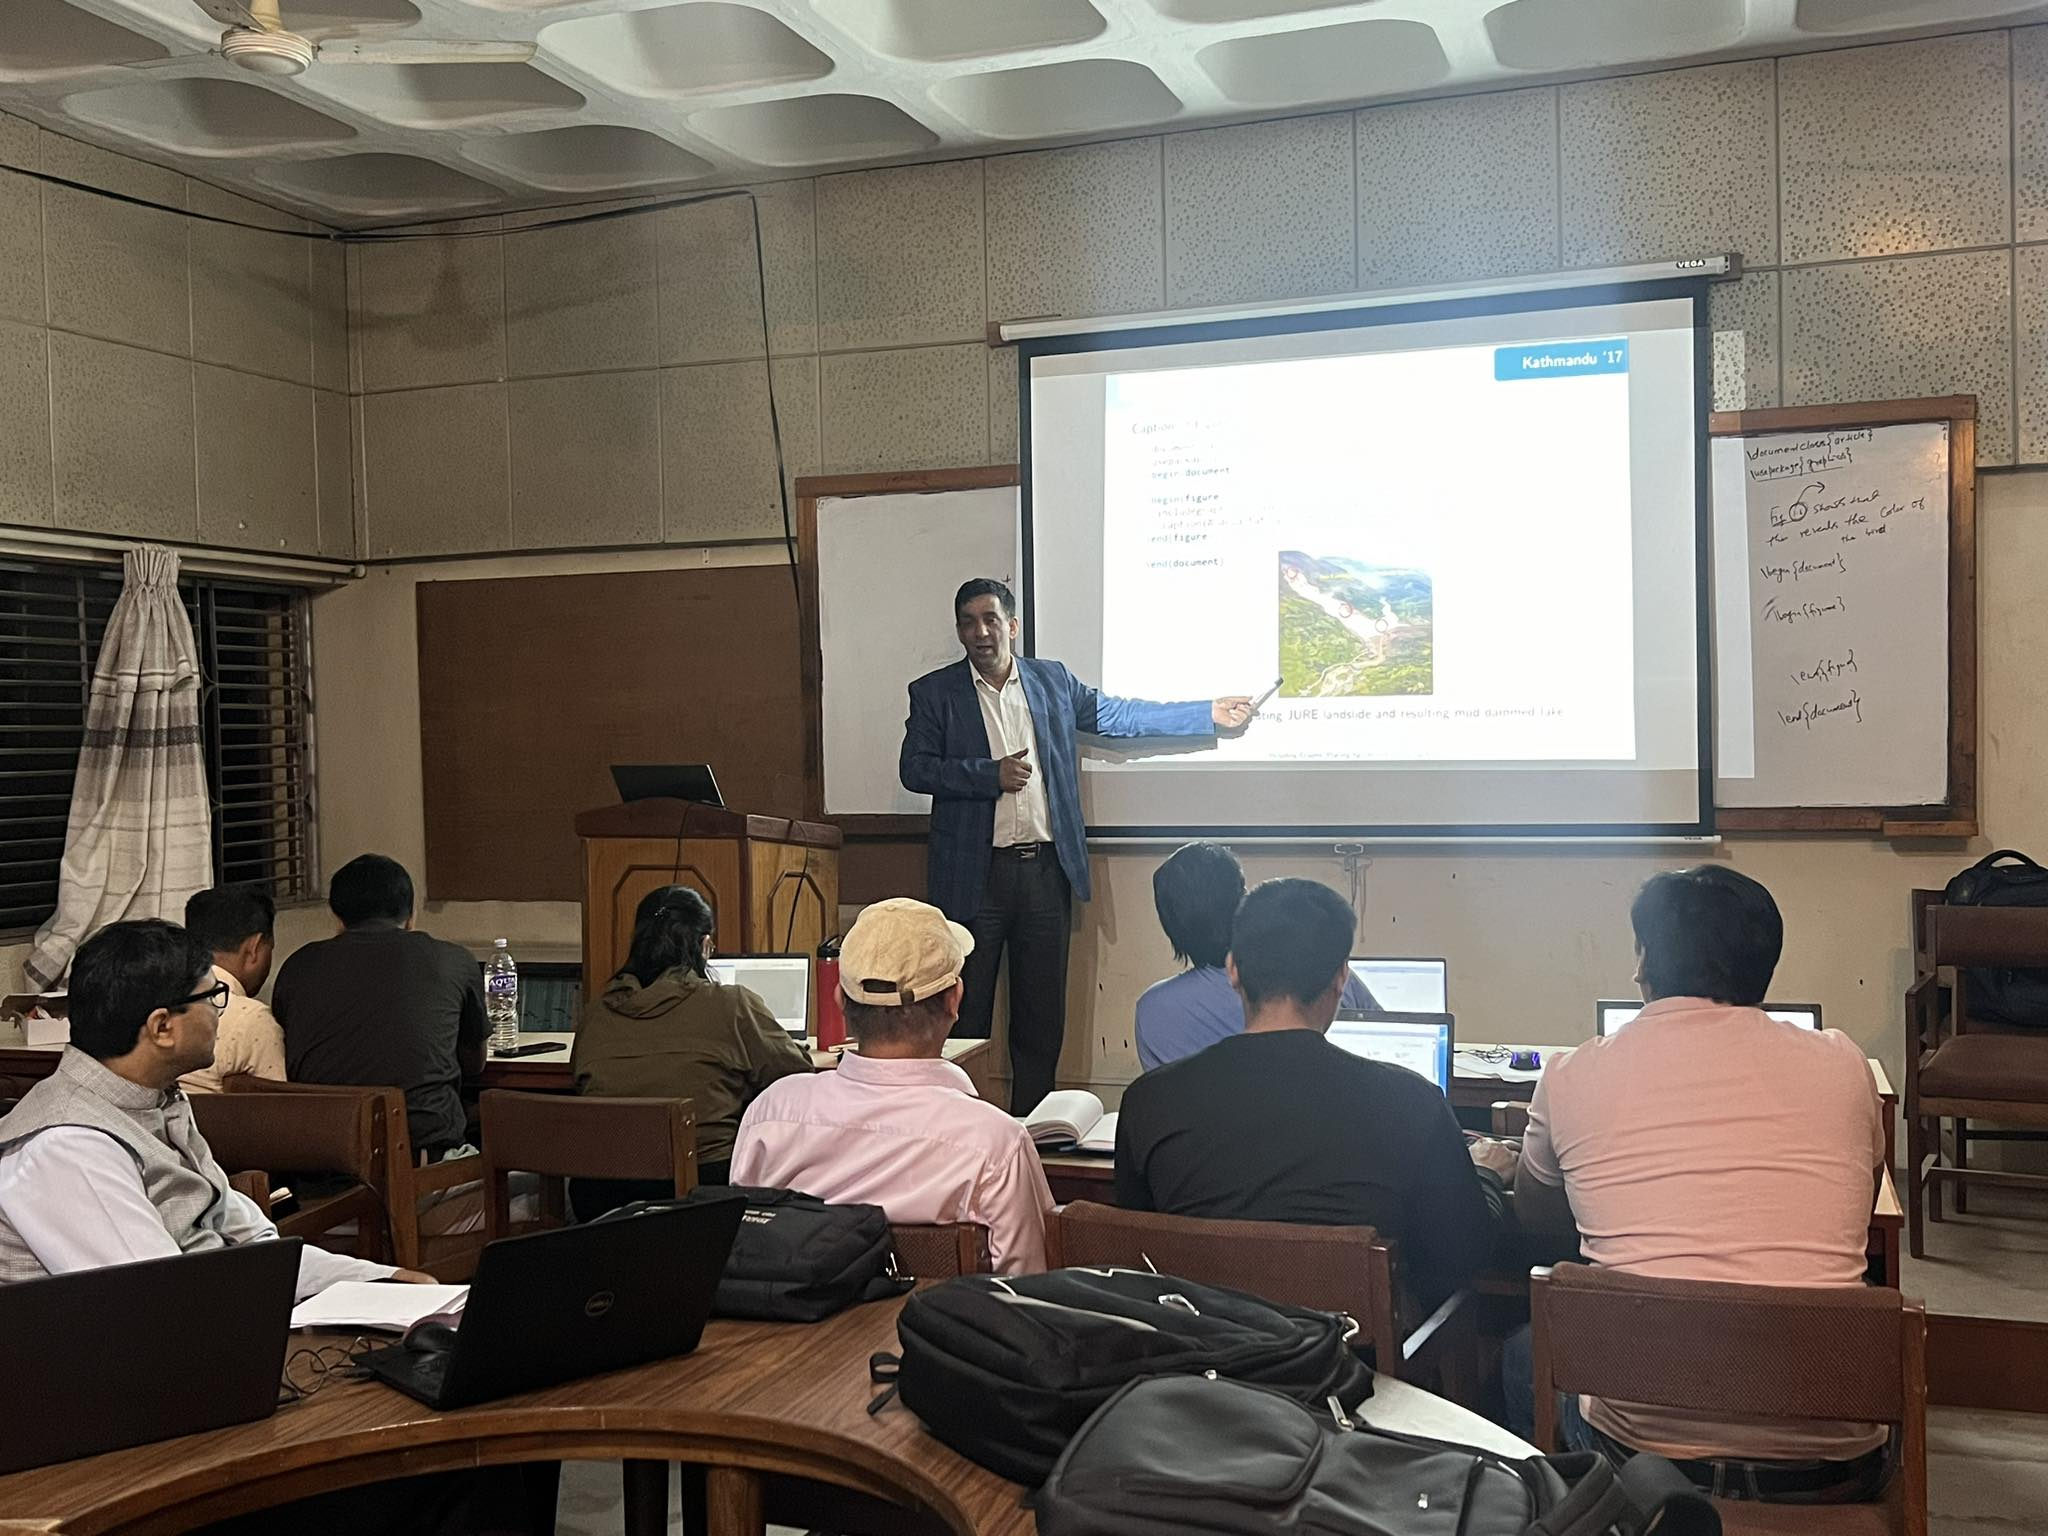
\includegraphics[height=7cm, width=9cm]{puskar.jpg}
  \caption{Dr. Puskar Raj Pokharel}
\end{figure}
\clearpage

\begin{center}
  {\bfseries \Large Day 2, 21-Baishakh, Friday}
\end{center}
\vspace{3mm}

{\bfseries \large Session 3 : Online session}\\[3mm]
The session was from 7pm to 9pm online. The special guest of this session was the principal of RR Campus, Dr. \textit{Jivan Jnawali}.  This session was done via zoom-meeting so it was open to all. The expert of this session was Dr. \textbf{Dil Bahadur Gurung} of School of Science, KU. He trained the participants on \textit{About the Template of the Nepali Mathematical Sciences Report /JNMS}. JNMS stands for Journal of Nepal Mathematical Society.

\begin{figure}[h!]
\centering
\begin{subfigure}{0.45\textwidth}
    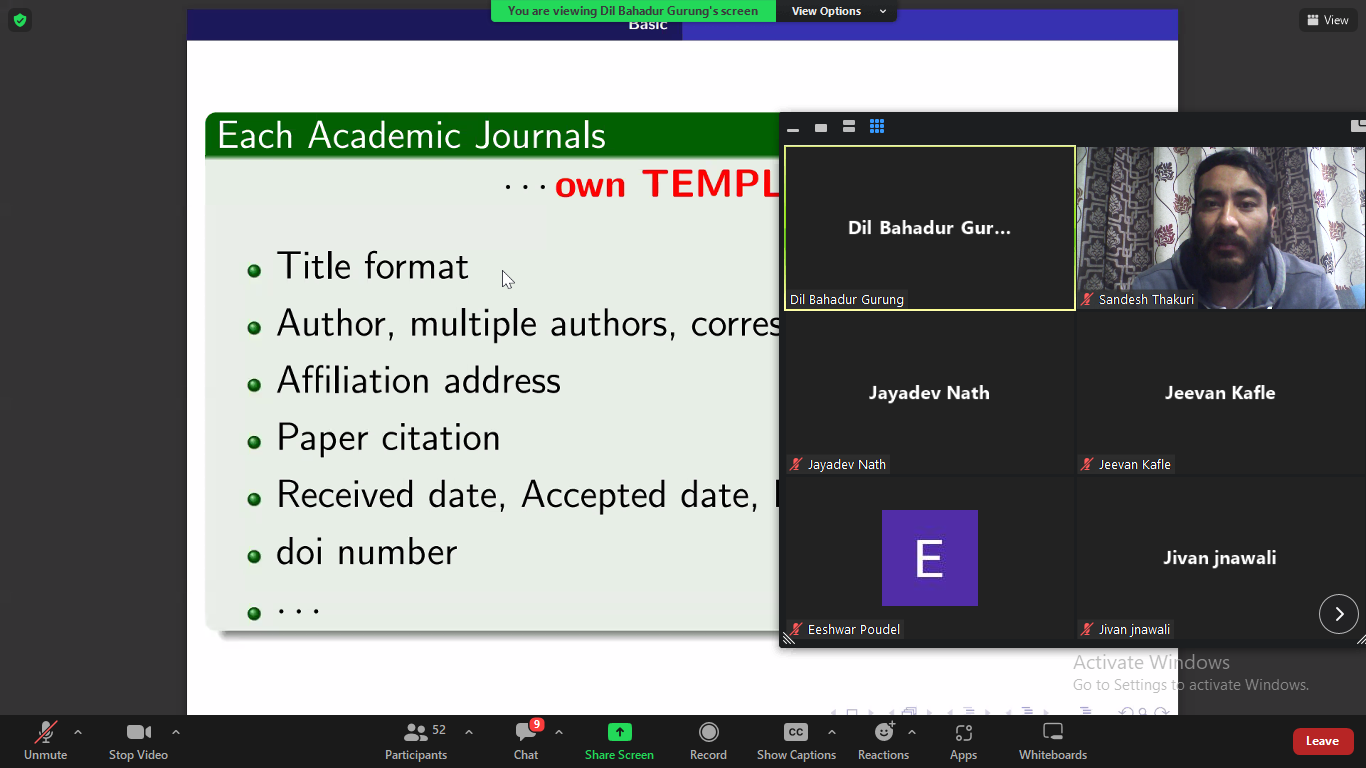
\includegraphics[height=5cm, width=\textwidth]{online1.png}
\end{subfigure}
\hfill
\begin{subfigure}{0.45\textwidth}
    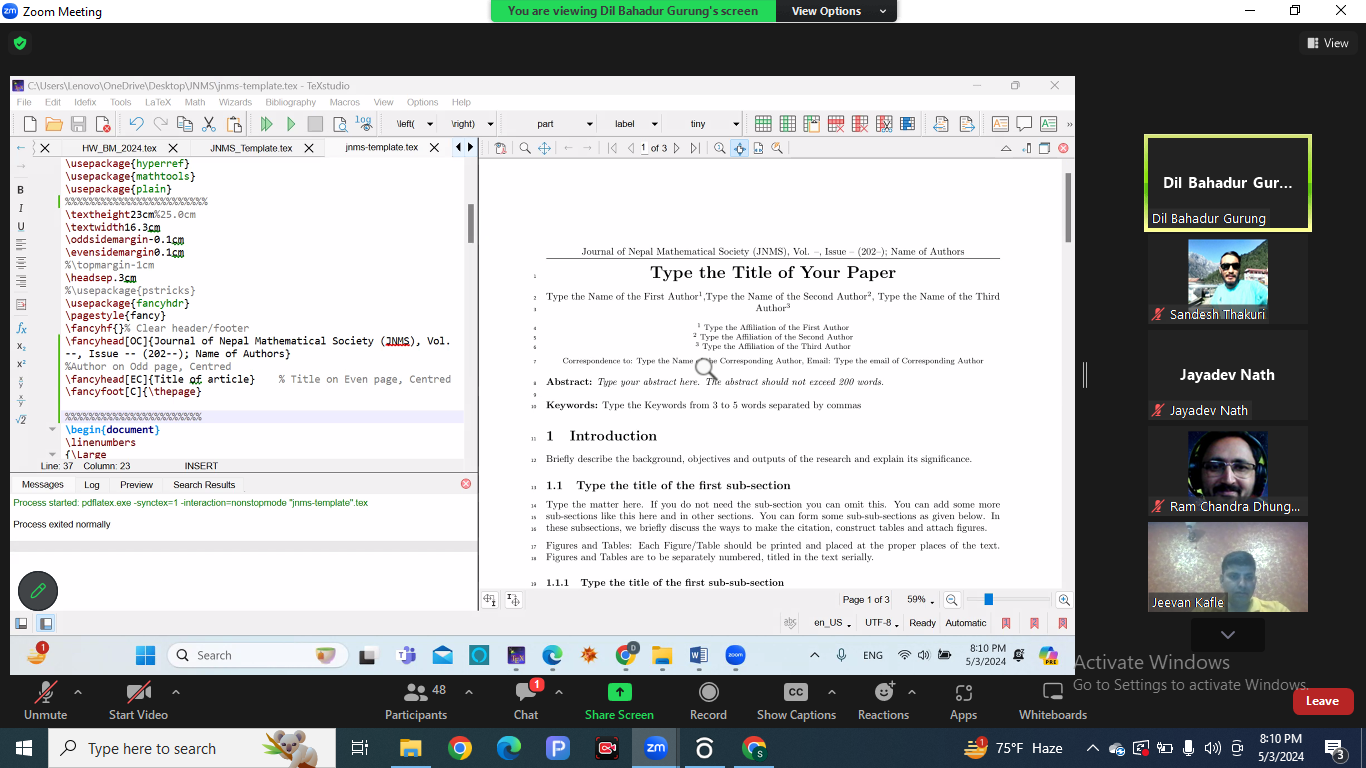
\includegraphics[height=5cm, width=\textwidth]{online2.png}
\end{subfigure}
\end{figure}

The templates of most scientific journals are done in latex including the JNMS. This is why latex is crucial. He mentioned that even a good research article may be rejected if not submitted in latex. He shared a story of his friend whose good research article was rejected simply because it was not done latex. He showed the participants the template of JNMS and instructed the participants the following.
Each journal has its own template. The template has its parts: Title, Author, Affiliation, Abstract, Main Body, Conclusion, Citation format etc. To format a article for a specific journal first visit its website and read the instructions for authors and download a latest article published to get the feel. Then download the template and work on it. Reference format and citation format are challenging aspects of article writing.
The session was ended with the questions from the participants and feedback from the special guest Dr. Jnawali.

\begin{figure}[h!]
  \centering
  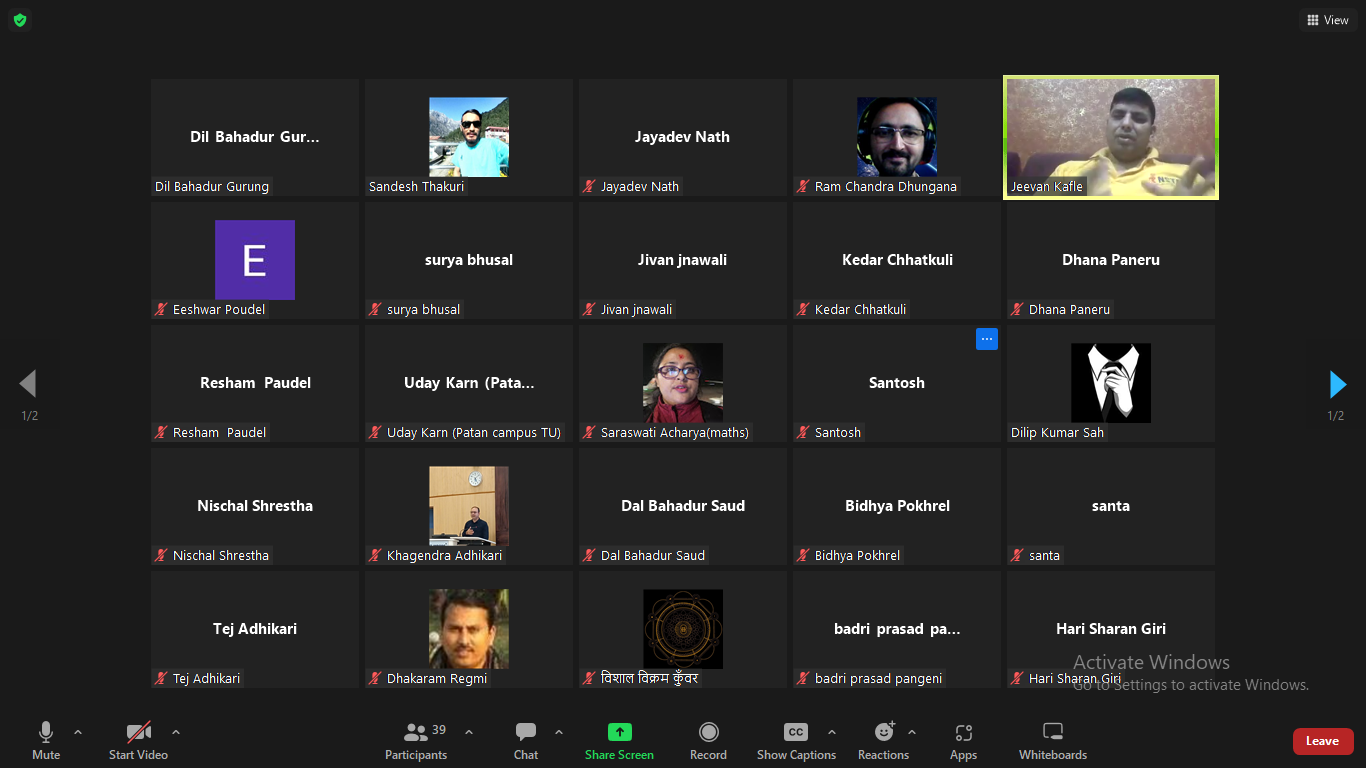
\includegraphics[height=7cm, width=15cm]{online3.png}
\end{figure}
\clearpage


\begin{center}
  {\bfseries \Large Day 3, 21-Baishakh, Saturday}
\end{center}
\vspace{3mm}

Before the fourth session Dr. Pokharel gave a quick revision to the participants from 11am to 12pm.\\

{\bfseries \large Session 4}\\[3mm]
The expert of this session was Dr. \textbf{Santosh Ghimire} of Pulchowk Campus, TU and Dr. \textbf{Kafle}. Dr. Ghimire trained the participants on \textit{Tabular Material and Document Layout}. First he taught the participants how to set the margins in a latex document which is generally done using the ``geometry package'' of the latex. This was followed by the document organization: chapter, section, subsection, paragraph, list, etc. Then he moved on to creating and placing of a tabular material in a latex document. Participants were given sufficient time to practice on their own. At ended he showed some tricks in latex. Mr. \textbf{Sandesh Thakuri} continued the session giving a talk on drawing graphics in latex using the package \textit{tikzpicture}. He made a flowchart using tikzpicture.
\vspace{7mm}

\begin{figure}[h!]
\centering
\begin{subfigure}{0.48\textwidth}
    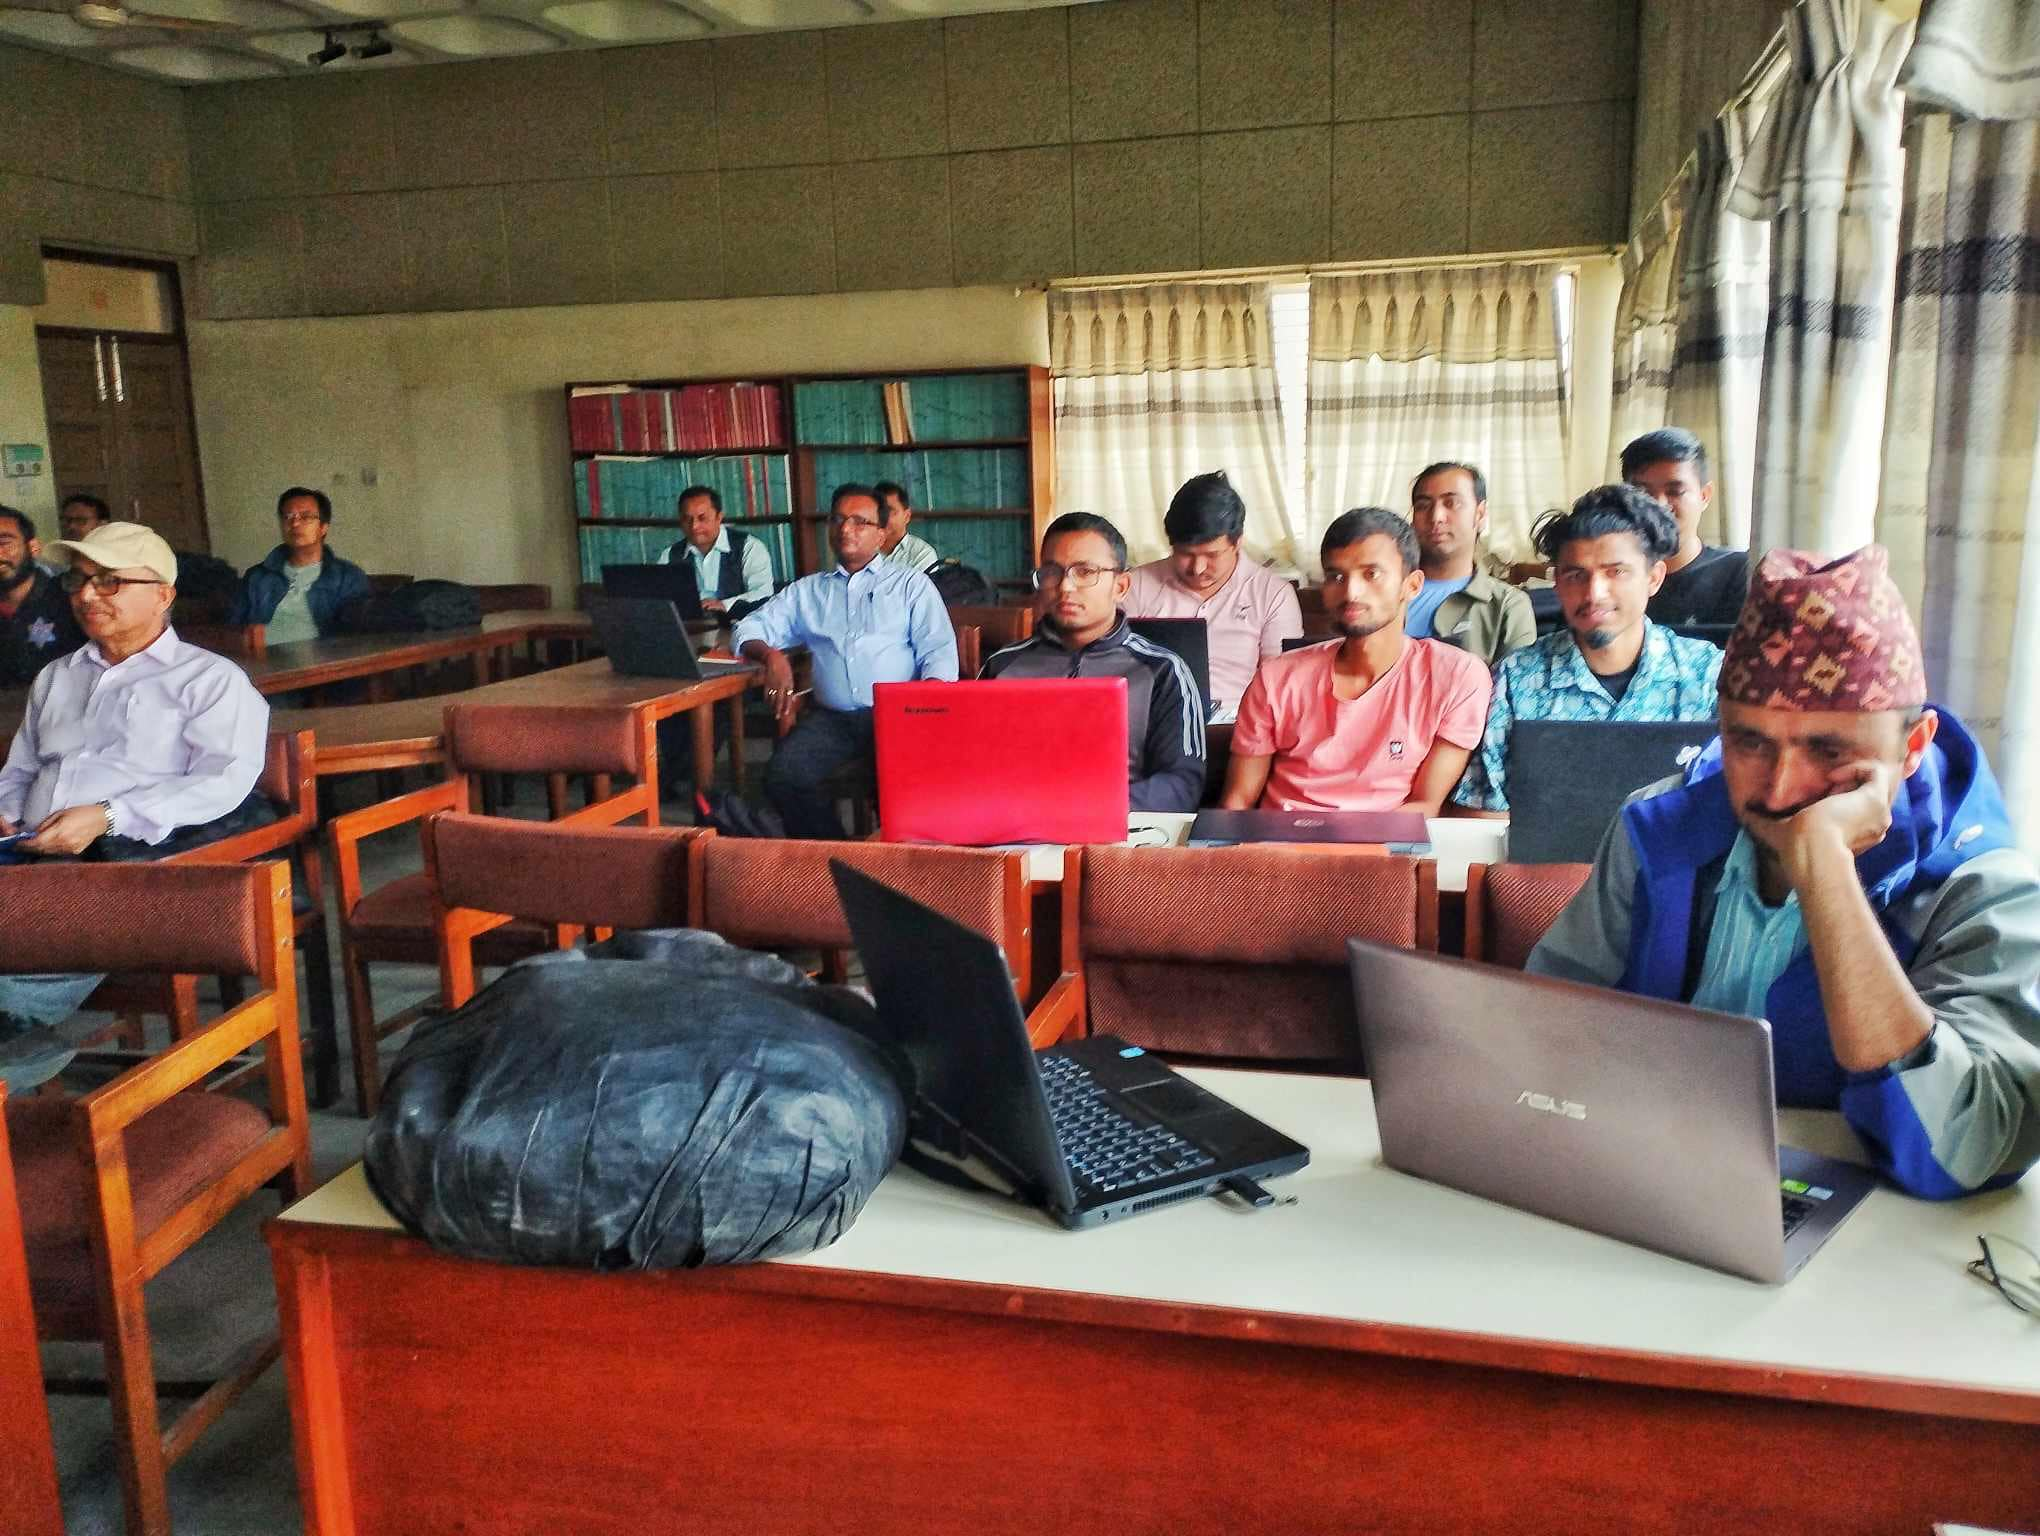
\includegraphics[height=6cm, width=\textwidth]{santosh.jpg}
\end{subfigure}
\hfill
\begin{subfigure}{0.48\textwidth}
    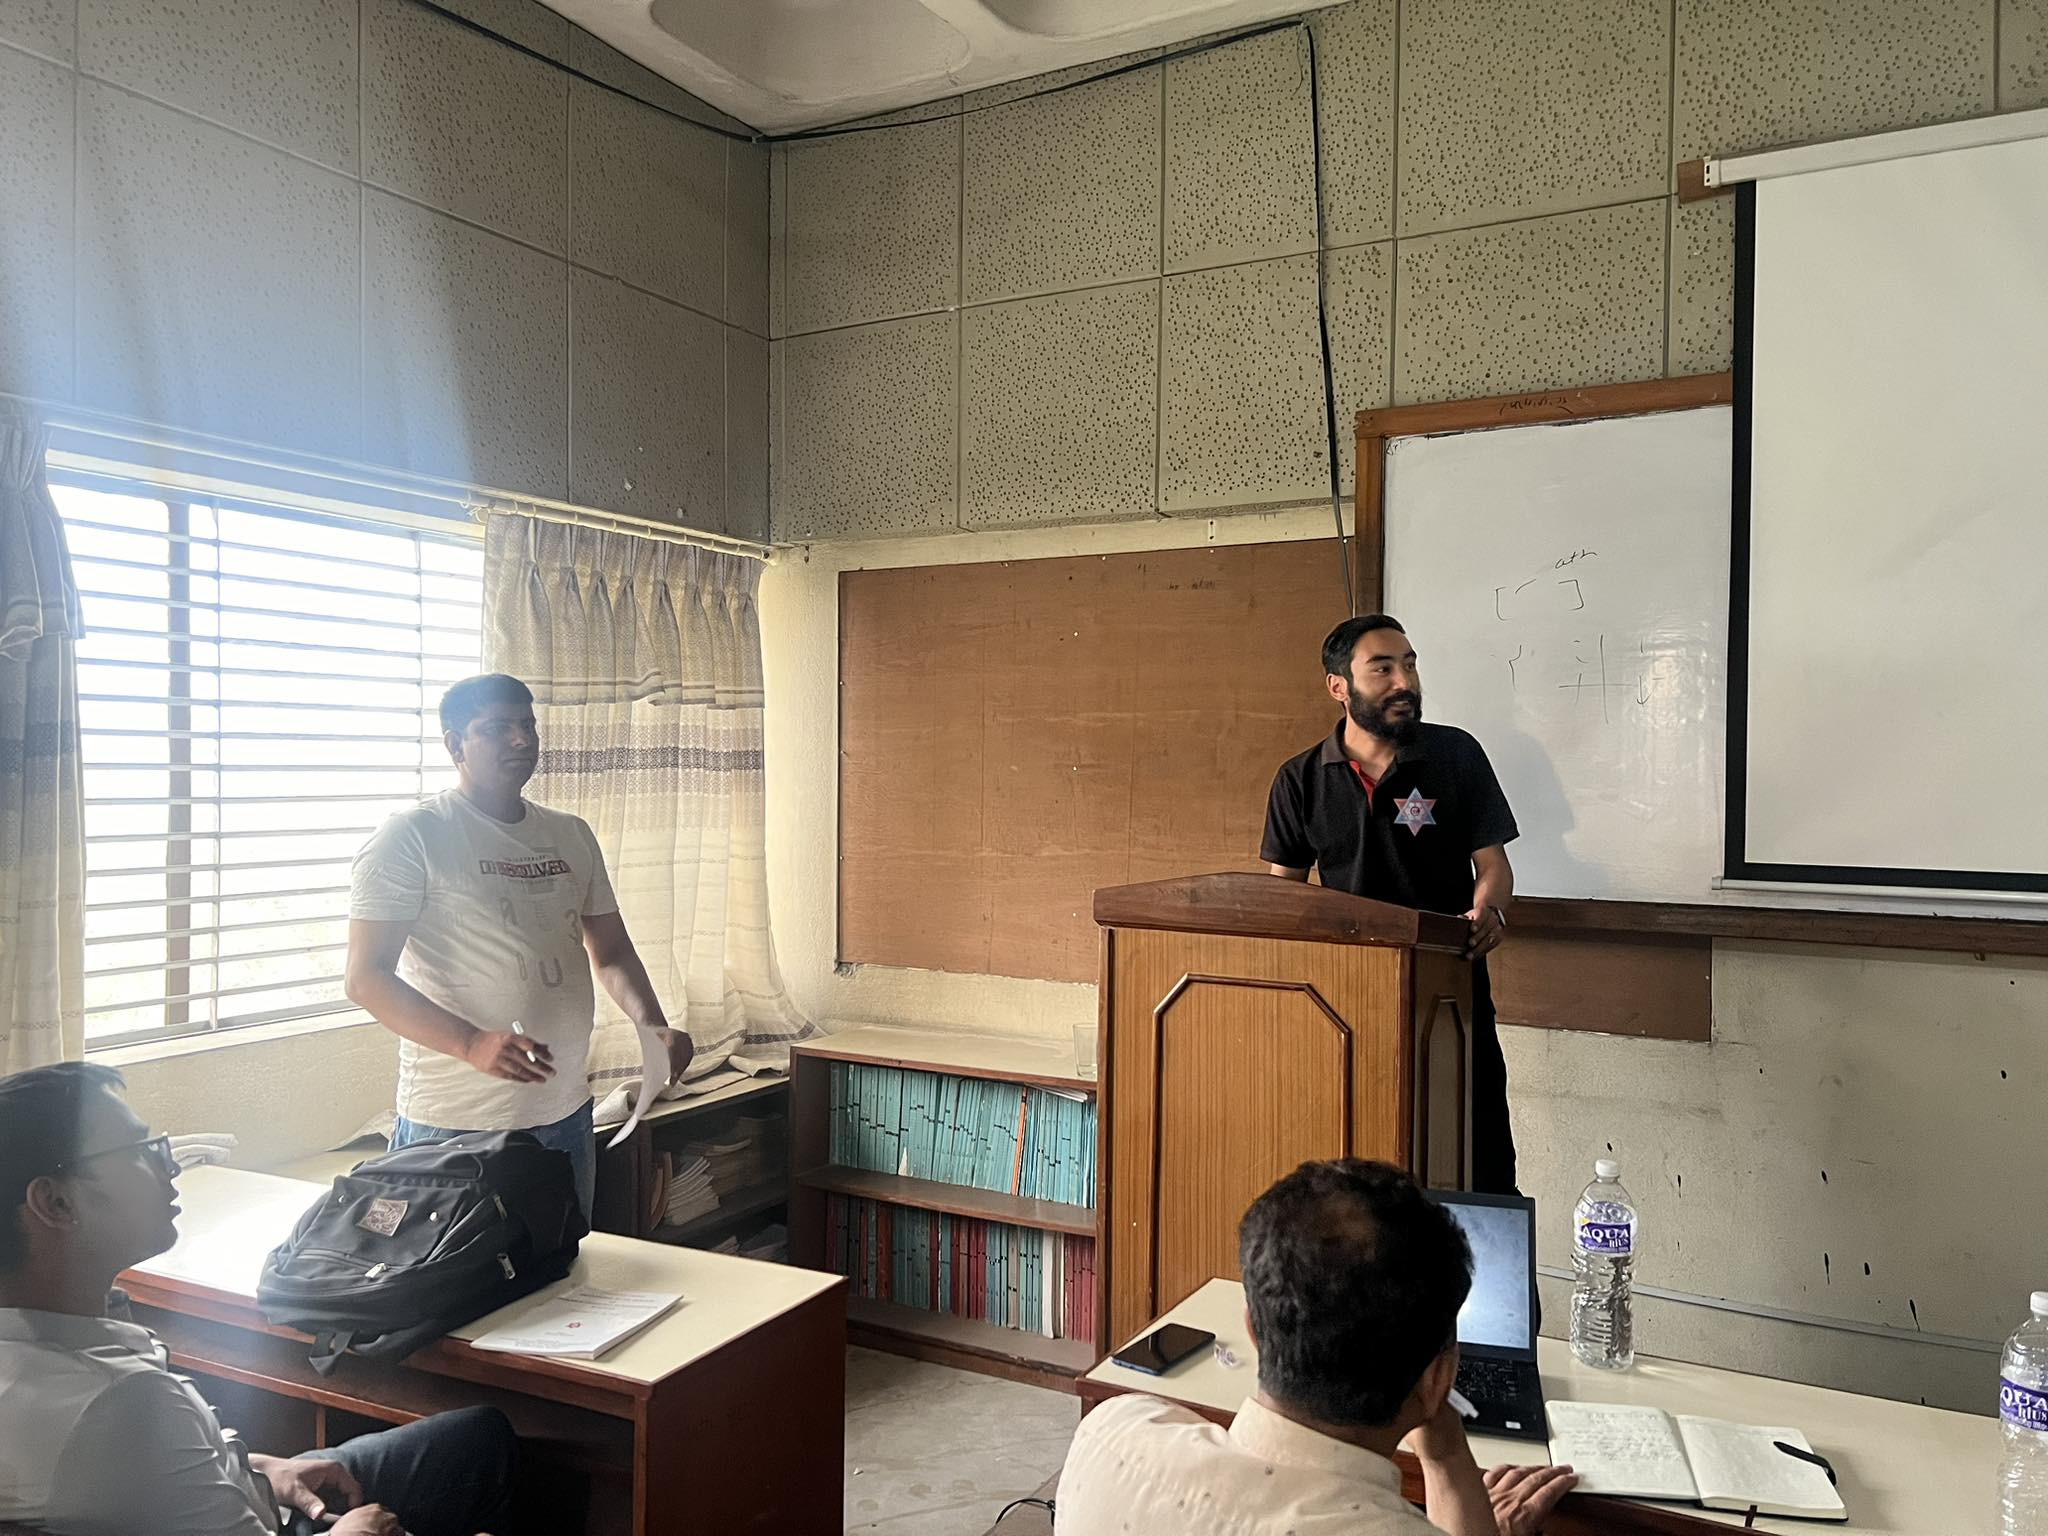
\includegraphics[height=6cm, width=\textwidth]{sandesh2.jpg}
\end{subfigure}
\end{figure}

\vspace{7mm}
{\bfseries \large Session 5}\\[3mm]
The expert of this session was Dr. \textbf{Dinesh Panthi} of Valmeeki Campus, Nepal Sanskrit University. Dr. Panthi trained the participants on \textit{Presentation in Beamer}. Beamer is a document class in latex. It allows us to create slides and frames which is a presentation tool in latex. This is a popular class used by the researchers to make a presentation. Dr. Panthi started with the \textit{preamble} of beamer class where title, author, institute, etc are set using which a title page is created. Then he taught on placing the a title pic and a logo in the presentation. He moved on to creating slides and frames and placing our contents on the frames. He ended the session with \textbf{overlays} in beamer which a crucial element of a presentation.
\clearpage

\vspace*{3mm}
\begin{center}
  {\bfseries \Large Closing Session}
\end{center}
\vspace{5mm}

{\bfseries \large Remarks by the Participants}\\[3mm]
To give a remark from the participants the president of the Student Council came forward. He remarked that the workshop has been very fruitful and has met all its objectives.\\[7mm]

{\bfseries \large Concluding Remarks}\\[3mm]
The special guest of the third day was secretary of Nepal Mathematical Society Assoc. Prof. Dr. \textbf{Prameshowri Kattel}. He was thrilled to know about the workshop and was in update about the workshop with Dr. Kafle. He shared his experience of learning and using latex. He and Dr. Kafle had learned it during their Phd in Kathmandu University. He said workshops as such are very helpful in sharing knowledge. He remarked that in eastern philosophy the we have a tradition of establishing a guru to a new thing and this workshop have facilitate as a guru for the latex learners.
\vspace{5mm}

\begin{figure}[h!]
\centering
\begin{subfigure}{0.45\textwidth}
  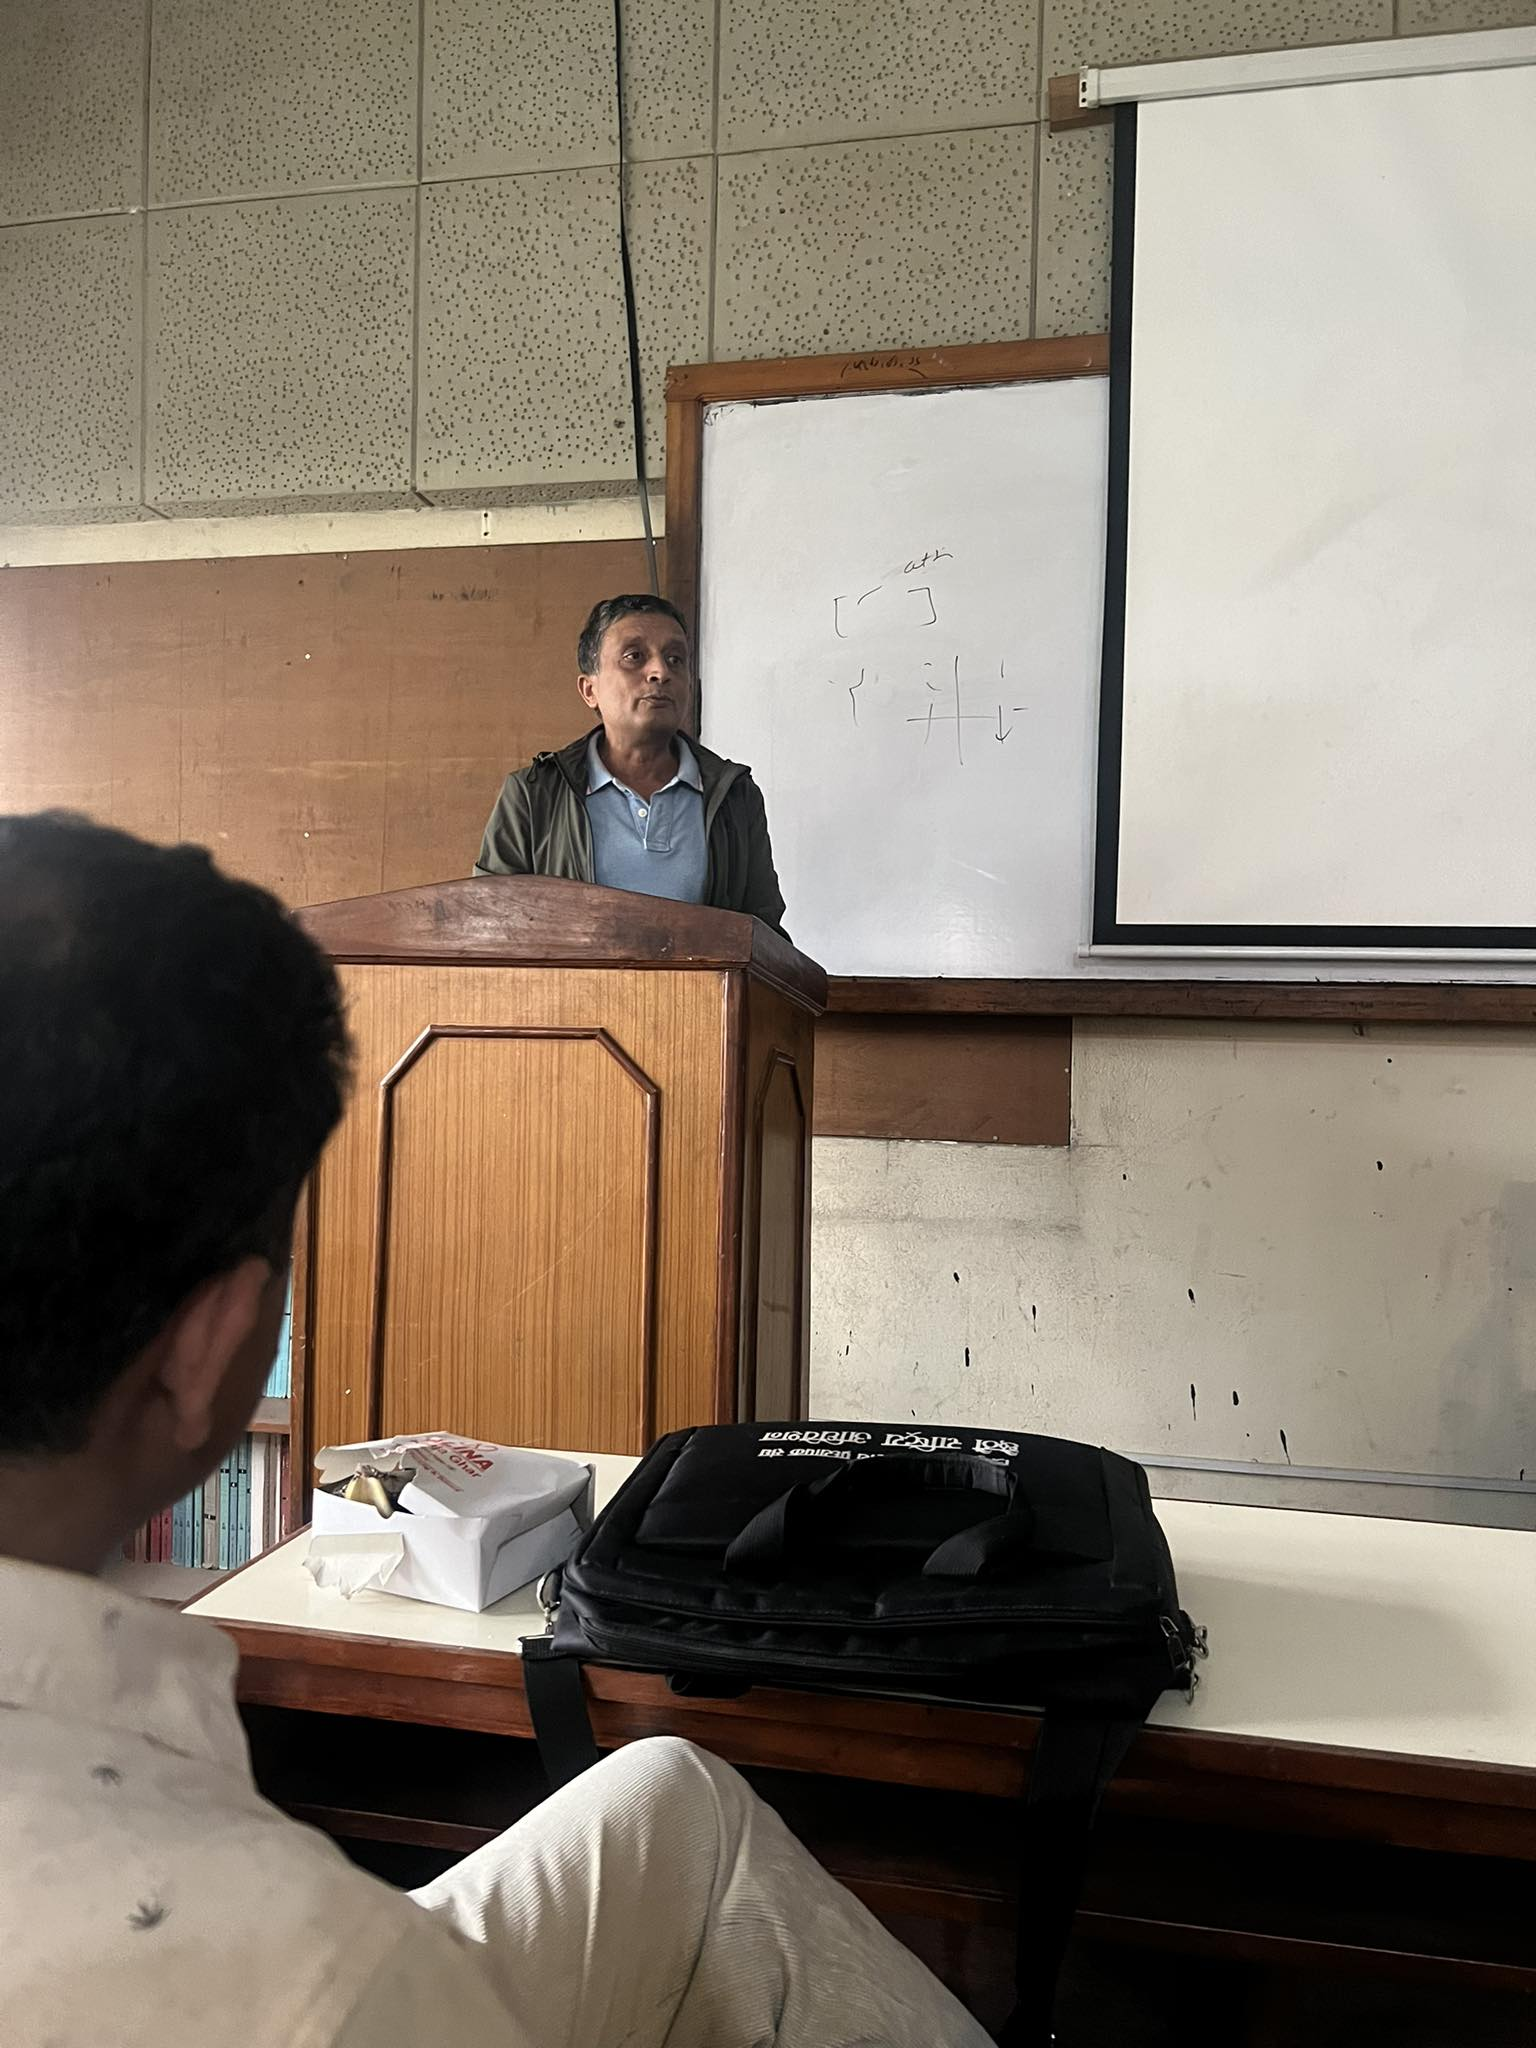
\includegraphics[height=7cm, width=\textwidth]{pramesh.jpg}
  \caption{Dr. Kattel}
\end{subfigure}
\hfill
\begin{subfigure}{0.45\textwidth}
  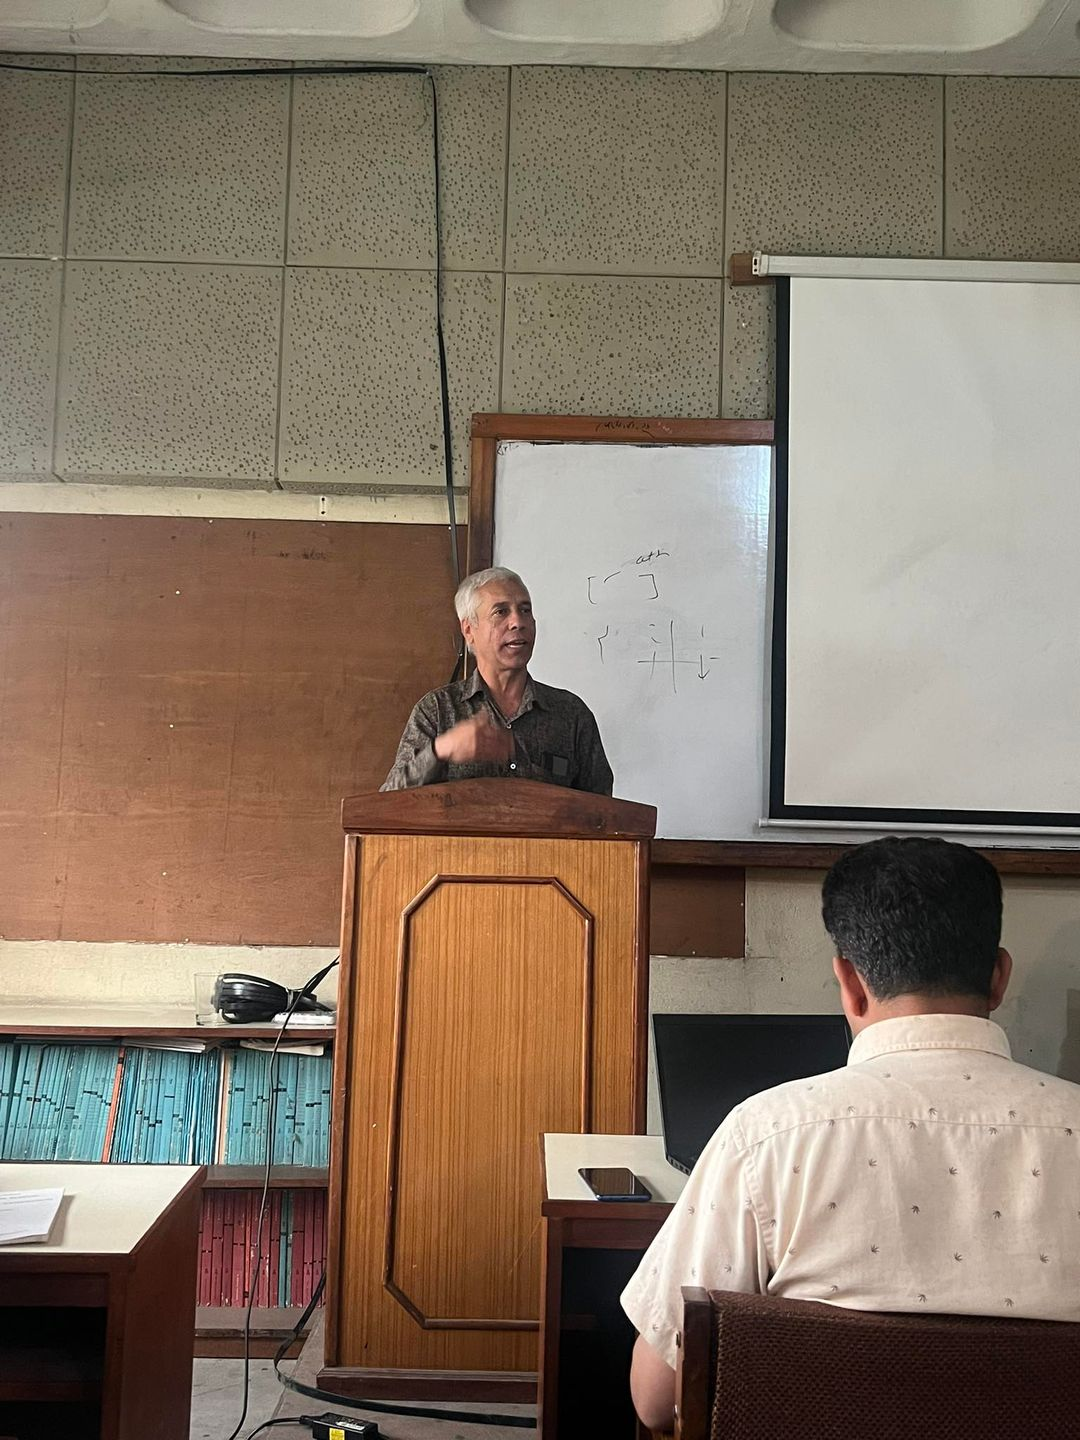
\includegraphics[height=7cm, width=\textwidth]{dinesh.jpg}
  \caption{Dr. Panthi}
\end{subfigure}
\end{figure}

\vspace{7mm}
Among the guests Dr. Panthi remarked success of the workshop and suggested the participants to keep practicing the latex to learn it well. Dr. Kafle the host and coordinator remarked that it is not possible to learn and understand everything about the latex in a single workshop. We have seen all the workings of the latex and must keep working on it on our own as well to fully master it. So one should not be dissapointed if there is some concept he/she has not understood fully. Finally he declared the conclusion of the workshop.
\clearpage


{\bfseries \large Token Love to the Guests}
\begin{figure}[h!]
\centering
\begin{subfigure}[c]{0.3\textwidth}
  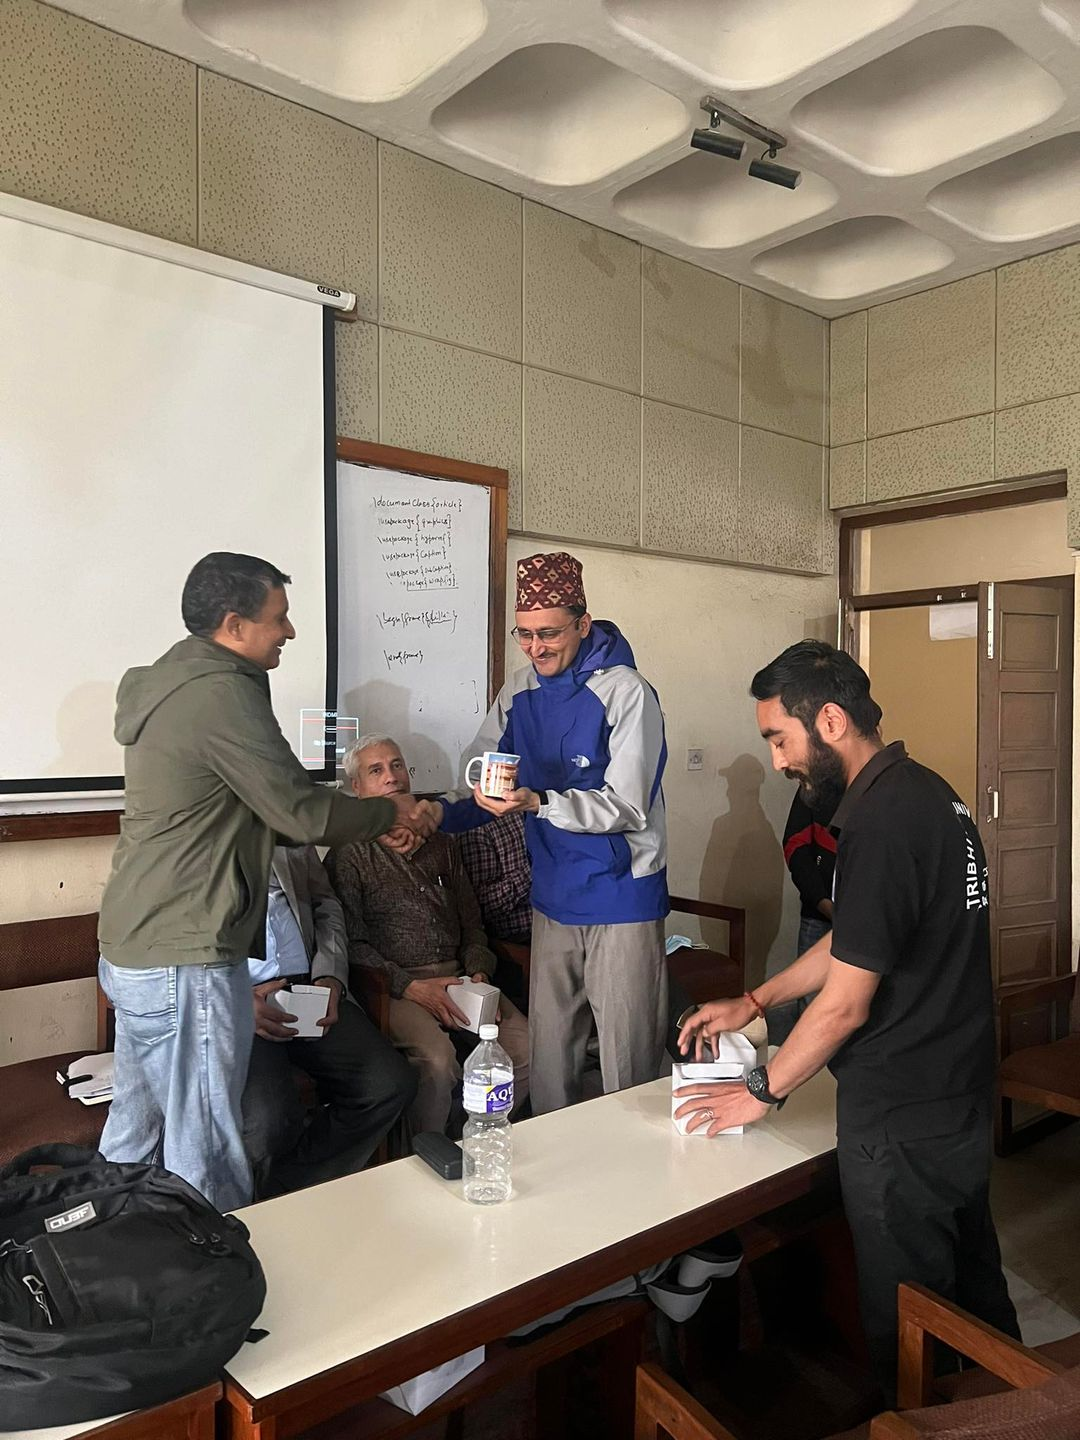
\includegraphics[height=6cm, width=\textwidth]{rcdt.jpg}
  \caption{Dr. Dhungana}
\end{subfigure}
\hfill
\begin{subfigure}[t]{0.3\textwidth}
  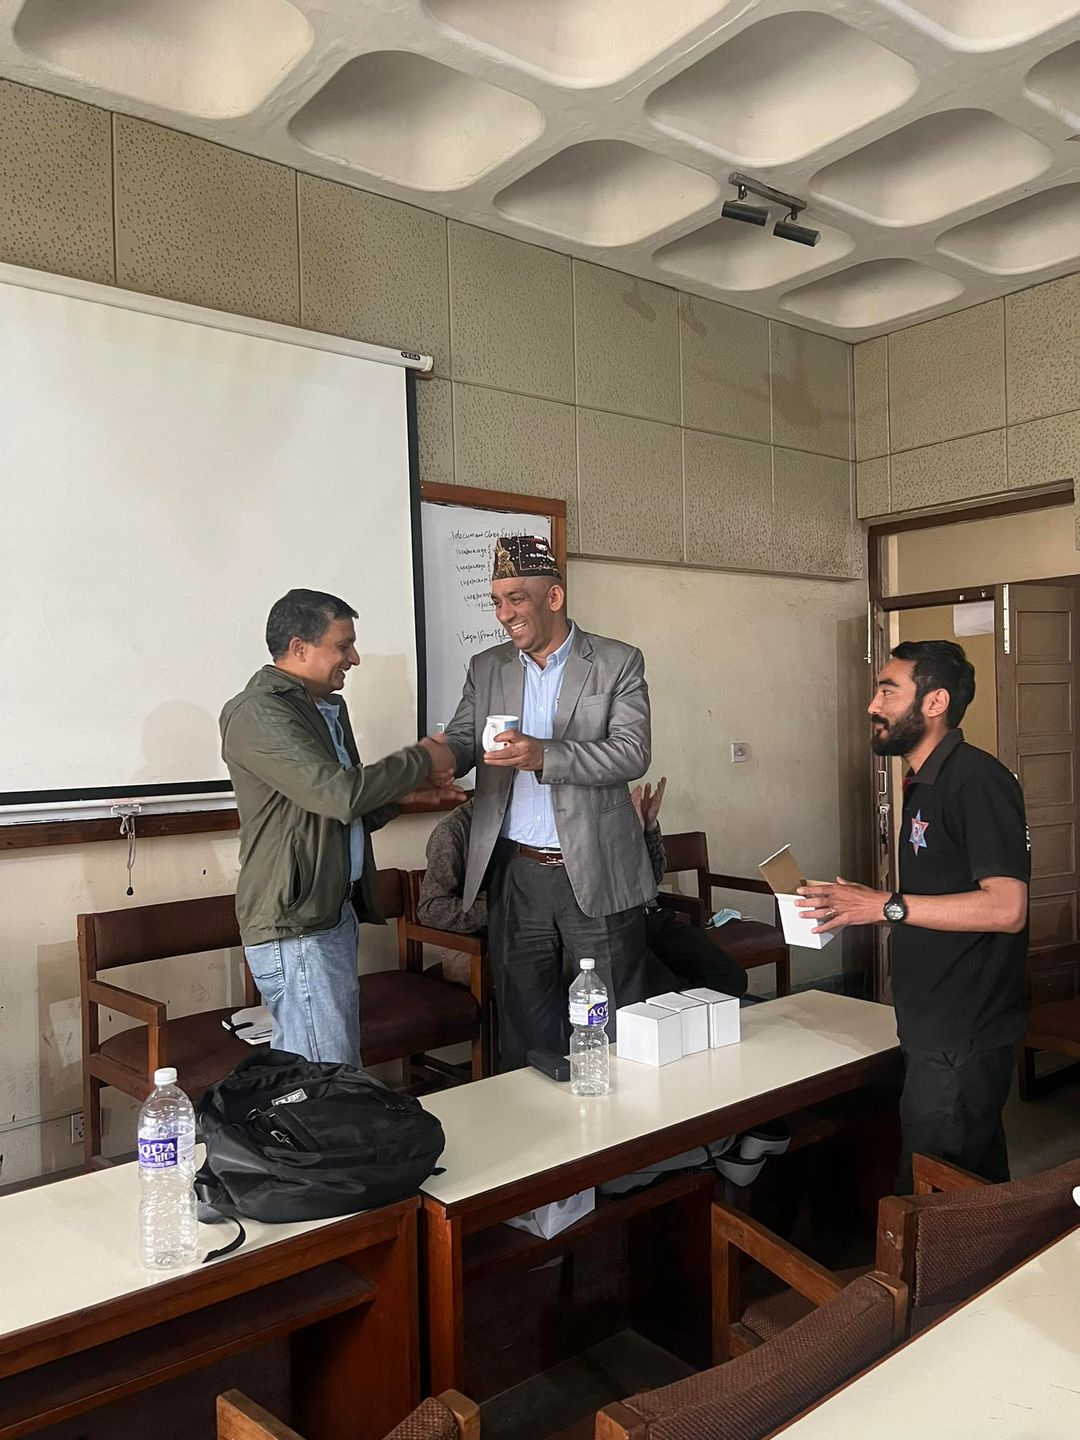
\includegraphics[height=6cm, width=\textwidth]{puskart.jpg}
  \caption{Dr. Pokharel}
\end{subfigure}
\hfill
\begin{subfigure}[b]{0.3\textwidth}
  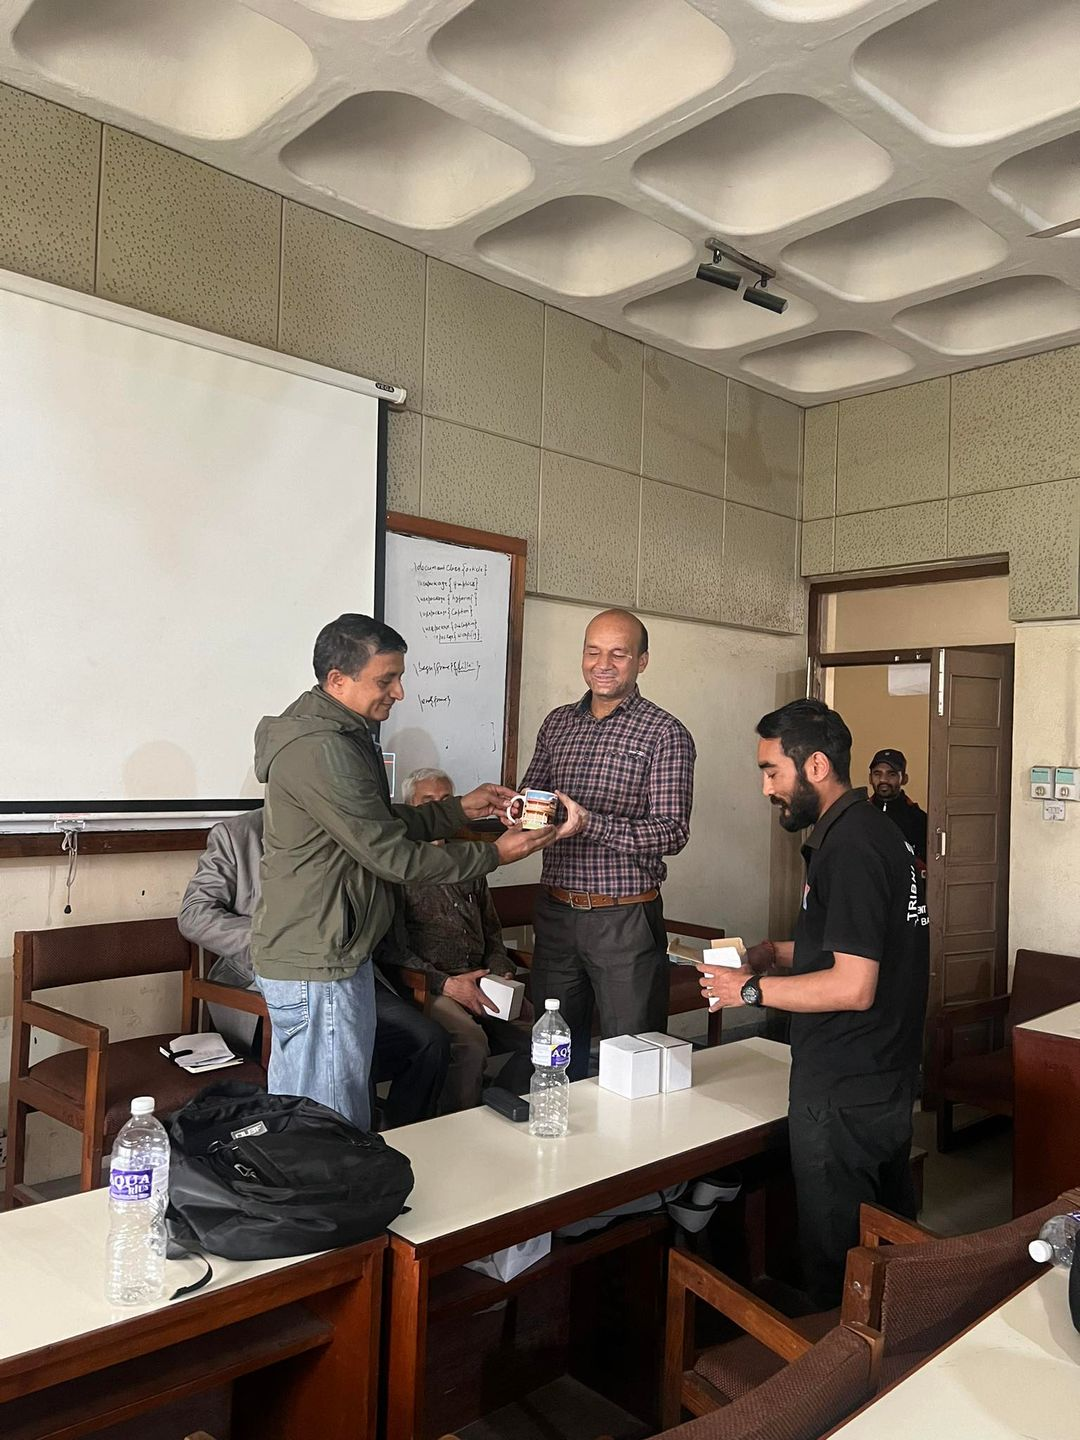
\includegraphics[height=6cm, width=\textwidth]{santosht.jpg}
  \caption{Dr. Ghimire}
\end{subfigure}
\end{figure}

{\bfseries \large Certificate Distribution Clips}

\begin{figure}[h!]
\message{ !name(latexworkhop_report.tex) !offset(123) }

\end{document}
%%% Local Variables:
%%% mode: latex
%%% TeX-master: t
%%% End:
